\section{D-RM Builder Tutorial}
\label{sec.drm.tut}
Several tutorials are given in this section to demonstrate the use of FOQUS to generate data-driven D-RMs.  The first tutorial contains general descriptions of the features and GUIs of the D-RM Builder, while the rest of the tutorials demonstrate the individual features and options.

Example files used for the tutorials are provided with the FOQUS installer and are typically installed at: C:\textbackslash Program Files (x86)\textbackslash foqus\textbackslash foqus\_2015.10.0\textbackslash examples\textbackslash DRMBuilder.  The three folders named VdV, pH, and BFB contain three ACM examples, one for each folder.  The folder named Matlab contains Matlab classes that represent D-RMs and a script to test generated D-RMs.

\subsection{Building Data-Driven D-RM using DABNet Framework and BP-Based ANN Training}
To demonstrate the feature, an example named Van-de-Vusse reactor is provided and installed in the VdV folder.  The nonlinear reactor model is a benchmark process popular in control literature.  The following are the steps to build a D-RM using DABNet framework and BP-based ANN training:
\begin{enumerate}
	\item Copy the ACM file of the Van-de-Vusse reactor ``VdV\_Reactor.acmf'' in ``C:\textbackslash Program Files (x86)\textbackslash foqus\textbackslash foqus\_2015.10.0\textbackslash examples\textbackslash DRMBuilder\textbackslash VdV'' to the FOQUS working directory.  Confirm the user of the D-RM Builder has write permissions to this folder.
	\item Launch SinterConfigGUI from Window$\text{'}$s ``Start'' menu or its shortcut on the desktop.  The GUI window as shown in Figure \ref{fig.sinter_gui_start} displays after a splash window.
	\begin{figure}[H]
		\begin{center}
			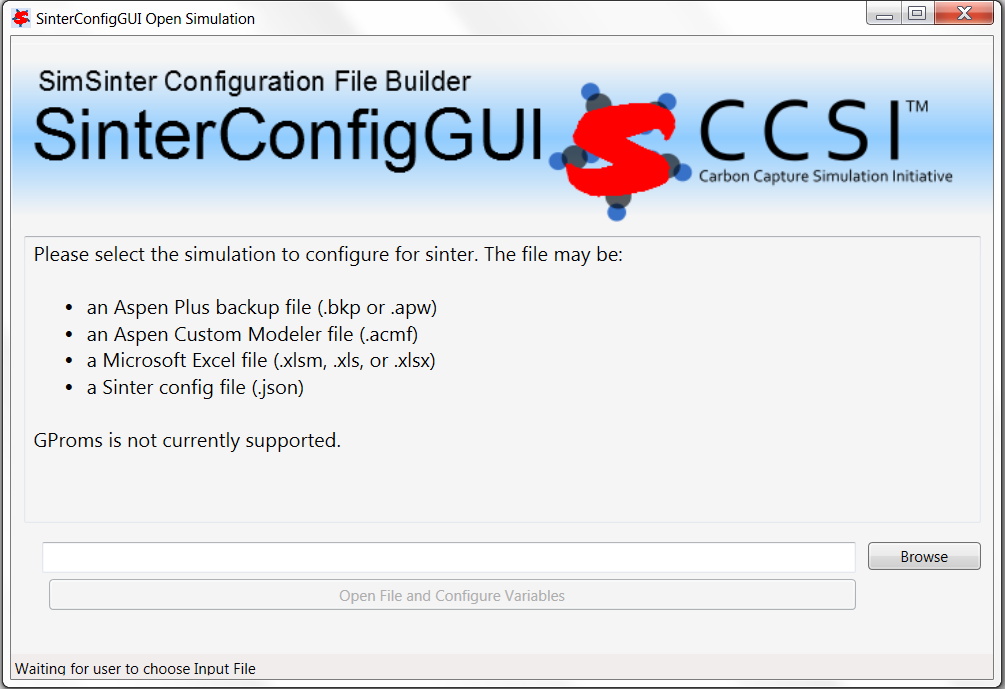
\includegraphics[scale=0.7]{Chapt_drm/figs/sinter_gui_start}
			\caption{Open Simulation Window for SinterConfigGUI}
			\label{fig.sinter_gui_start}
		\end{center}
	\end{figure}
	\item Click the \textbf{\underline{Browse}} button and browse to the ``VdV\_Reactor.acmf'' file in the working directory.  Then click the \textbf{\underline{Open File and Configure Variables}} button.  It takes a few seconds for the SinterConfigGUI to display a ``SinterGonfigGUI Simulation Meta-Data'' window as shown in Figure \ref{fig.sinter_gui_meta_data}.  An ACM window with VdV reactor model inside also displays as shown in Figure \ref{fig.sinter_gui_acm_vdv}.
	\begin{figure}[H]
		\begin{center}
			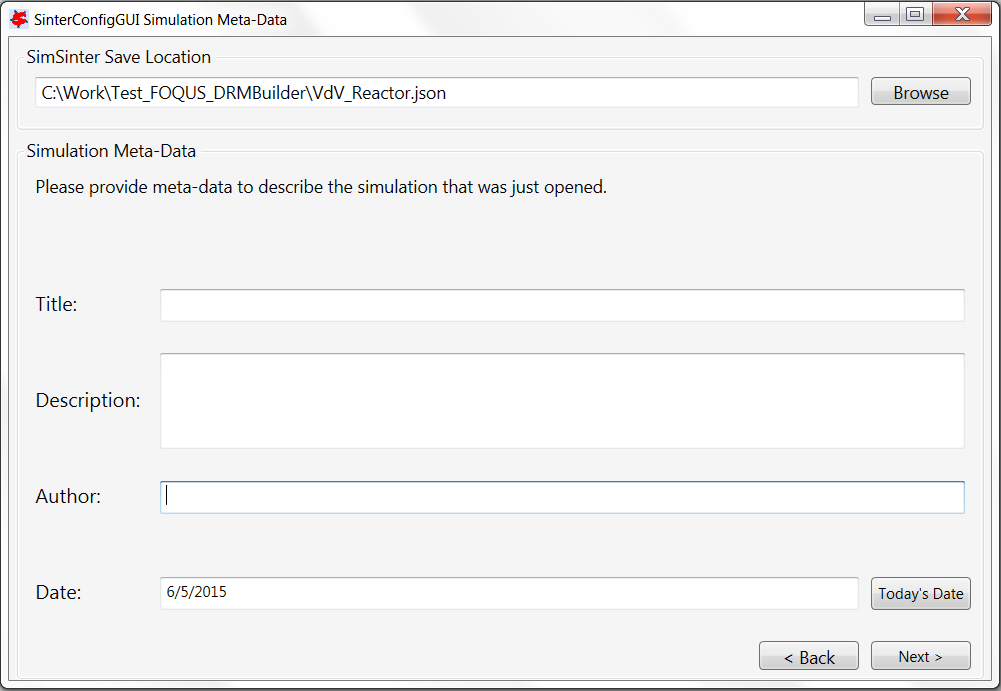
\includegraphics[scale=0.7]{Chapt_drm/figs/sinter_gui_meta_data}
			\caption{Dialog Window for the Simulation Meta-Data of VdV Reactor Model}
			\label{fig.sinter_gui_meta_data}
		\end{center}
	\end{figure}
	\begin{figure}[H]
		\begin{center}
			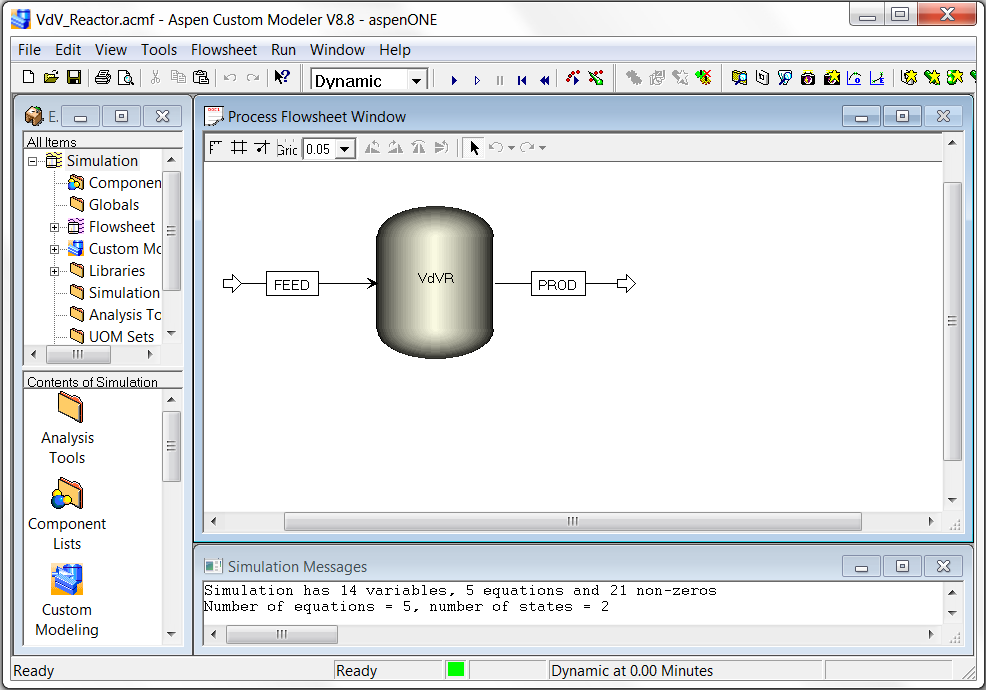
\includegraphics[scale=0.7]{Chapt_drm/figs/sinter_gui_acm_vdv}
			\caption{ACM Window Displayed for VdV Reactor Model by SinterConfigGUI}
			\label{fig.sinter_gui_acm_vdv}
		\end{center}
	\end{figure}
	\item Enter ``VdV Reactor Example'' in the \textbf{\underline{Title}} text box, ``My first DRMBuilder tutorial'' in the \textbf{\underline{Description}} text box, and user's name in the \textbf{\underline{Author}} text box.  Then click the \textbf{\underline{Next}} button.  A ``SinterConfigGUI Variable Configuration Page'' window displays as shown in Figure \ref{fig.sinter_gui_variable_config}.
	\begin{figure}[H]
		\begin{center}
			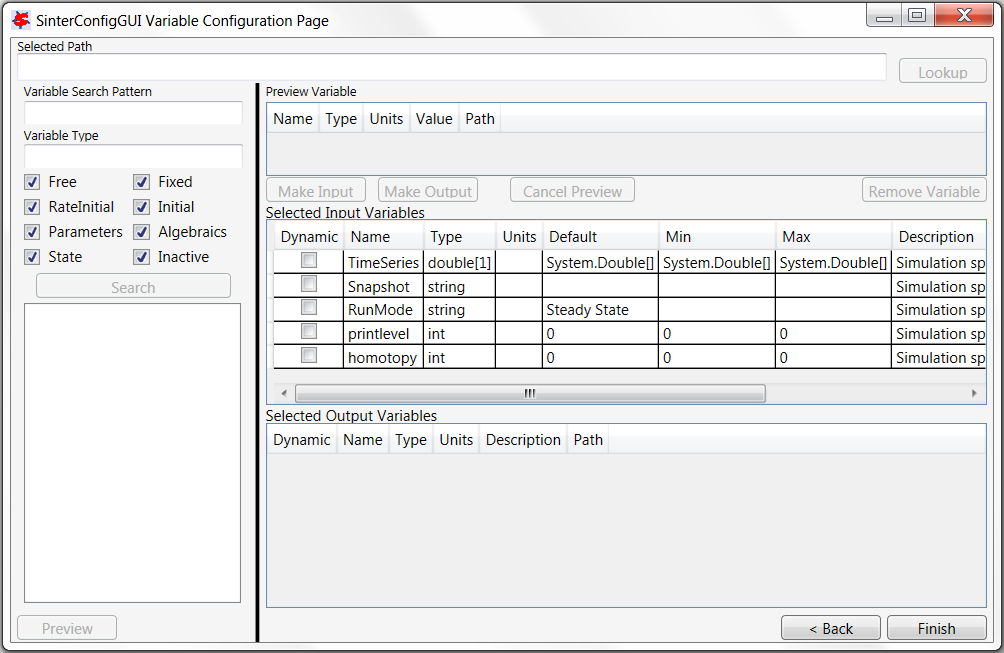
\includegraphics[scale=0.7]{Chapt_drm/figs/sinter_gui_variable_config}
			\caption{Variable Configuration Page of SinterConfigGUI}
			\label{fig.sinter_gui_variable_config}
		\end{center}
	\end{figure}
	\item Enter ``$\sim$'' in the \textbf{\underline{Variable Search Pattern}} text box and click the \textbf{\underline{Search}} button.  All of the variables in the VdV reactor model are listed in the list box at the lower left corner of the window as shown in Figure \ref{fig.sinter_gui_search}.
	\begin{figure}[H]
		\begin{center}
			\includegraphics[scale=0.7]{Chapt_drm/figs/sinter_gui_search}
			\caption{Variable List on Configuration Page of SinterConfigGUI}
			\label{fig.sinter_gui_search}
		\end{center}
	\end{figure}
	\item Select the ``VdVR.Feed.Ca'' in the list box and click the \textbf{\underline{Lookup}} button at the upper right corner.  The variable is displayed in the ``Preview Variable'' section.  Click the \textbf{\underline{Make Input}} button and the variable is appended to the end of the ``Selected Input Variables'' table.  Change the name of the variable to ``Ca\_Feed'' and select the checkbox in the \textbf{\underline{Dynamic}} column.  This makes the selected variable a dynamic input variable.
	\item Select the ``VdVR.Feed.F'' in the list box and repeat Step 6 to make it a dynamic input variable and change the name to ``F\_Feed''.
	\item Select the ``VdVR.V'' in the list box and repeat Step 6 to make it a dynamic input variable and change the name to ``V\_Reactor''.
	\item Change the default value of the input variable named ``RunMode'' in the ``Selected Input Variables'' table from ``Steady State'' to ``Dynamic''.  Please do not enter quotes.
	\item Select the ``VdVR.Prod.Ca'' in the list box and click the \textbf{\underline{Preview}} button.  Then click the \textbf{\underline{Make Output}} button and the variable is added to the ``Selected Output Variables'' table.  Change the name of the variable to ``Ca\_Product'' and select the checkbox in the \textbf{\underline{Dynamic}} column.  This makes the selected variable a dynamic output variable.
	\item Select the ``VdVR.Prod.Cb'' in the list box and repeat Step 10 to make it a dynamic output variable and change the name to ``Cb\_Product''.
	\item This concludes the configuration of ACM variables.  Figure \ref{fig.sinter_gui_final} shows the SinterConfigGUI window after the configuration.  Click the \textbf{\underline{Next}} button at the lower right corner and a ``SinterConfigGUI Vector Default Initialization'' dialog window displays as shown in Figure \ref{fig.sinter_gui_vector}.  Leave the default time series data unchanged. 
	\begin{figure}[H]
		\begin{center}
			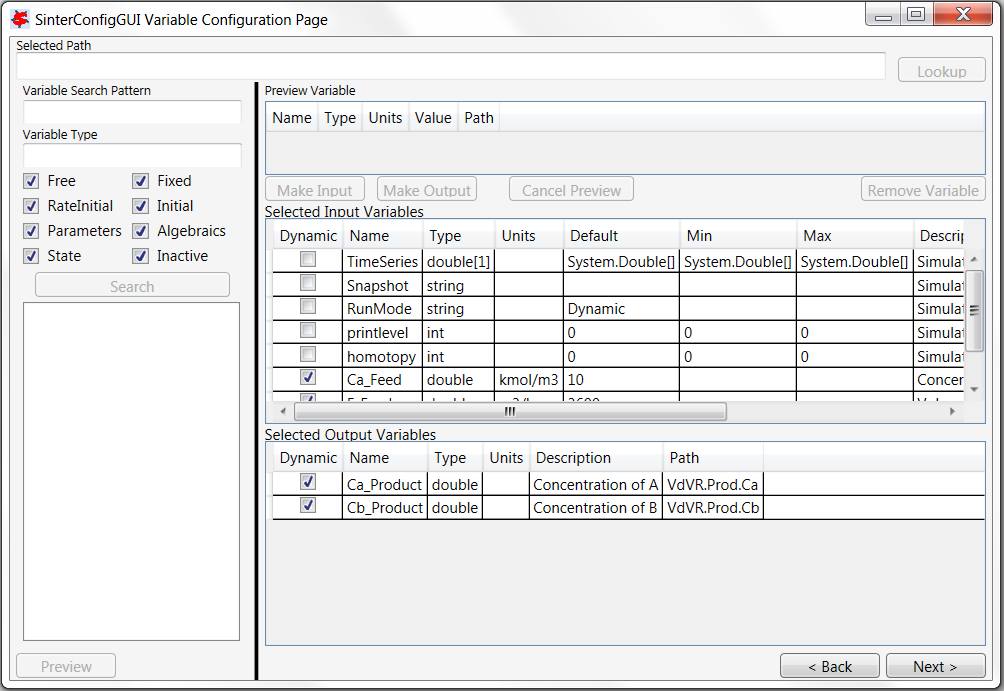
\includegraphics[scale=0.7]{Chapt_drm/figs/sinter_gui_final}
			\caption{Configured Dynamic Variables by SinterConfigGUI}
			\label{fig.sinter_gui_final}
		\end{center}
	\end{figure}
	\begin{figure}[H]
		\begin{center}
			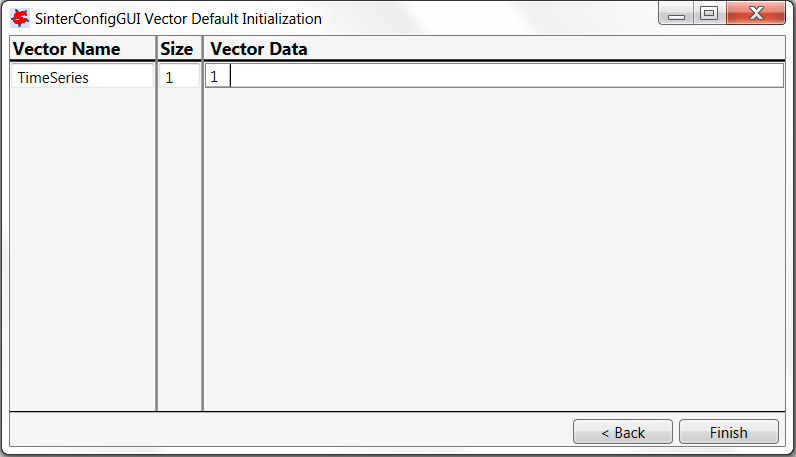
\includegraphics[scale=0.7]{Chapt_drm/figs/sinter_gui_vector}
			\caption{Time Series Vector Specification Window of SinterConfigGUI}
			\label{fig.sinter_gui_vector}
		\end{center}
	\end{figure}
	\item Click the \textbf{\underline{Finish}} button to exit the ``SinterConfigGUI''.  A file named ``VdV\_Reactor.json'' is created in the working directory.  Close the ACM window.
	\item After the dynamic input and output variables are configured and the JSON file is created, start FOQUS.  The main window of the FOQUS displays.  Click the \textbf{\underline{Settings}} icon 
\includegraphics[scale=0.7]{Chapt_drm/figs/drm_icon_settings} and make sure the ``SimSinter Home'' is set to the full path of the folder (not a file inside the folder) where SinterConfigGUI.exe is located.  Click the \textbf{\underline{DRM-Builder}} icon \includegraphics[scale=0.7]{Chapt_drm/figs/drm_icon_drmbuilder} and the embedded D-RM Builder frame displays as shown in Figure \ref{fig.drm_start}.
	\begin{figure}[H]
		\begin{center}
			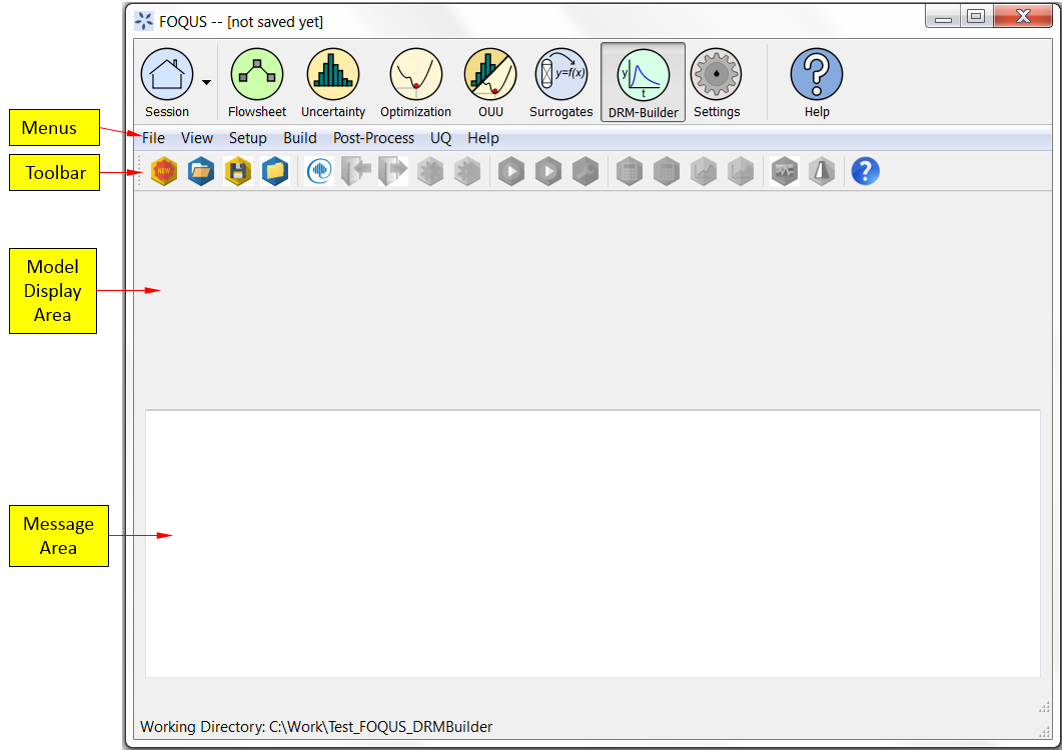
\includegraphics[scale=0.7]{Chapt_drm/figs/drm_start}
			\caption{Embedded D-RM Builder Window with a Blank D-RM Project}
			\label{fig.drm_start}
		\end{center}
	\end{figure}
	\item The embedded D-RM Builder widget is similar to a classical Microsoft Windows application with menus and a toolbar at the top, a gray area for displaying the input and output variables (initially blank), a client area with white background in the middle, and a status bar at the bottom.  The client area is used to display the messages.  Browse the individual menus to see the submenus or commands.  Some of the submenus are shaded (disabled) initially.  They are enabled later when the status of the D-RM building process is updated.  When the mouse is moved over a menu or a toolbar icon, a tip about the command displays over the menu or icon while a short description about the command displays in the status bar at the bottom of the embedded window.  If a menu ends with ``...'', it brings up a dialog window for more user inputs.  Initially a blank project exists in the FOQUS framework and the user can start to work on the blank project by choosing a high-fidelity model (ACM model) configured in Steps 1--13 through the \textbf{\underline{Setup}} menu.  The \textbf{\underline{File}} menu contains ``New'', ``Open'', ``Close'', ``Save'', ``Save As'', and ``Export'' submenus.  Add a new case to the main window by issuing the \textbf{File $\rightarrow$ New} command or clicking on the toolbar icon 
\includegraphics[scale=0.15]{Chapt_drm/figs/new}.  If the current project is not saved, the D-RM Builder will ask the user to save the project.  Open an existing case by issuing the \textbf{File $\rightarrow$ Open} command or clicking the toolbar icon 
\includegraphics[scale=0.15]{Chapt_drm/figs/open}.  Again, the D-RM Builder will ask the user to save the project if the current project has been modified.  Close the current case by issuing the \textbf{File $\rightarrow$ Close} command or clicking the toolbar icon \includegraphics[scale=0.25]{Chapt_drm/figs/close} and a blank project will be displayed.  Save a case by issuing the \textbf{File $\rightarrow$ Save} command or clicking the toolbar icon 
\includegraphics[scale=0.25]{Chapt_drm/figs/save}.  Save a case to a different name by issuing the \textbf{File $\rightarrow$ Save As} command.  The typical workflow for building and testing a D-RM is from the \textbf{\underline{Setup}} menu, to the \textbf{\underline{Build}} menu, the \textbf{\underline{Post-Process}} menu, and finally to the \textbf{\underline{UQ}} menu (from left to right).  Within each menu, the general workflow is from the top command (submenu) to the bottom command.  The \textbf{\underline{File}} menu handles typical file opening, saving, and exporting commands, which could be issued at any time.  Depending on the status of the D-RM building process, the user may or may not export certain files under the \textbf{File $\rightarrow$ Export} command.  The toolbar icons are arranged from left to right following the typical D-RM building workflow.
	\item To start the D-RM building process for a blank case, select a high-fidelity model first.  Issue \textbf{Setup $\rightarrow$ Choose High-Fidelity Model} command or click the toolbar icon \includegraphics[scale=0.12]{Chapt_drm/figs/aspen_tech}.  A ``SimSinter Configuration File'' window displays for file browsing and selecting.  Browse and select the ``VdV\_Reactor.json'' file created in Step 12.  This loads the configuration file into the D-RM Builder.  A text message confirming the file selection and loading displays in the client area of the D-RM Builder window.
	\item The SinterConfigGUI allows a user to select the dynamic input and output variables.  Further configuration among the selected input and output variables are required to setup the D-RM Builder project.  To configure the selected ACM input variables, navigate to the \textbf{Setup $\rightarrow$ Configure Input Variables} command or click the toolbar icon \includegraphics[scale=0.15]{Chapt_drm/figs/config_input}.  The ``Input Variable Dialog'' window displays as shown in Figure \ref{fig.drm_input_variable_dlg}.
	\begin{figure}[H]
		\begin{center}
			\includegraphics[scale=0.7]{Chapt_drm/figs/drm_input_variable_dlg}
			\caption{Input Variable Dialog Window for VdV\_Reactor Model}
			\label{fig.drm_input_variable_dlg}
		\end{center}
	\end{figure}
	The input variables are listed in the ``Input Variable List'' list box.  Note: The order of the variables listed is not necessarily the order listed in SinterConfigGUI. The user can change the order of the input variables in the list by clicking the \textbf{\underline{Up}} and \textbf{\underline{Down}} arrow buttons near the right side of the list box.  For this tutorial, leave the order unchanged.  Click each of the variables to see the description, unit, and default ranges (±10\%) used for conducting training/validation.  The \textbf{\underline{Name}} and \textbf{\underline{Unit}} text boxes are for read-only.  The name of the variable here represents an ACM's internal variable path with a local variable name appended to a block name.  If the input variable is dimensionless, a space is displayed in the \textbf{\underline{Unit}} text box.  The user can edit the \textbf{\underline{Description}} text box as desired.  For each input, define whether or not it is included in the D-RM.  If excluded, the input variable is assumed to be constant and does not change with time.  This can be useful for cases where the user wants to use an input as an unmodeled/unknown disturbance or where an input is a fixed parameter.  In this example, the second input (``V\_Reactor'') represents the volume of the reactor and is never going to change in the course of the dynamic runs.  Therefore, specify the input as a time-invariant input by clearing the \textbf{\underline{Varies With Time}} check box (make sure the other two inputs are selected).  The total number of variables with their \textbf{\underline{Varies With Time}} check box selected is displayed in the read-only \textbf{\underline{Number of Time Dependent Variables}} text box.  Another specification, the \textbf{\underline{Use Ramp To Replace Step Change}} option is not used in this example (keep this check box cleared for all three inputs).  This option is used and discussed in the BFB example.  Also notice that when the \textbf{\underline{Varies With Time}} check box is cleared, the \textbf{\underline{Lower Limit}}, \textbf\underline{{Upper Limit}}, and \textbf{\underline{Ramp Rate}} text boxes and the \textbf{\underline{Use Ramp To Replace Step Change}} check box are disabled.  When the \textbf{\underline{Varies With Time}} check box is selected, the user can change the lower and upper limits of the variable to desired values.  However, the lower limit cannot be larger than the default value displayed at the read-only \textbf{\underline{Default}} text box, which is usually the steady-state value used in the original ACM model.  Likewise, the upper limit cannot be smaller than the default value.  If this rule is broken, a warning message dialog box displays when the user clicks \textbf{\underline{OK}} and the user cannot exit the dialog box unless the user clicks \textbf{\underline{Cancel}}, which cancels all of the values and options that the user has entered on the ``Input Variable Dialog'' window.  For this example, leave the default values of the lower and upper limits for the input variables unchanged.


	Depending on the time scale of the system response, the user may need to revise the sampling time interval, which is the time interval that is used in the discrete-time D-RM.  The sampling time interval should be comparable with the time constants of the output variables in response to the change of input variables.  The \textbf{\underline{Solver Minimum Time}} step label displays the minimum integration time step used by the ACM solver.  The sampling time interval should be higher than the solver minimum time step.  The \textbf{\underline{Time Step During Ramp}} is not applicable in this case since no ramp change is used.  If the ramp changes are used to replace step input changes, the \textbf{\underline{Time Step During Ramp}} needs to be specified to a value that is greater than the minimum solver time step and less than the sampling time interval.  Leave the default sampling time interval of 0.01 hours unchanged.  Click \textbf{\underline{OK}} to accept the new configured values and close the ``Input Variable Dialog'' window.  The messages in the client area confirm that the input variables are properly specified for the D-RM.  Two arrows connected to a black box are plotted in the upper half of the D-RM Builder window, representing the two input variables.
	\item Configure the output variables by issuing the \textbf{Setup $\rightarrow$ Configure Output Variables} command or clicking the toolbar icon 
\includegraphics[scale=0.2]{Chapt_drm/figs/config_output}.  The ``Output Variable Dialog'' window as shown in Figure \ref{fig.drm_output_variable_dlg} displays.  
	\begin{figure}[H]
		\begin{center}
			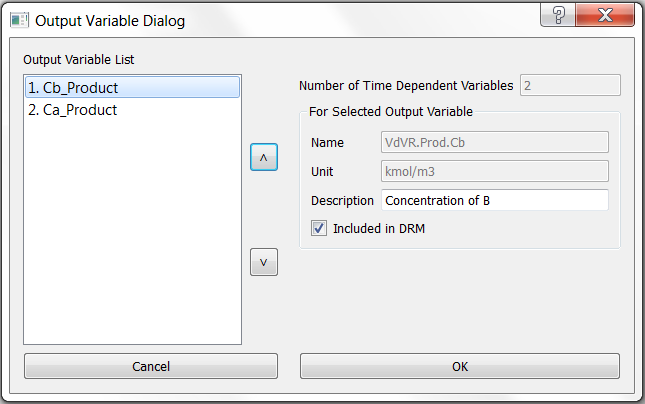
\includegraphics[scale=0.7]{Chapt_drm/figs/drm_output_variable_dlg}
			\caption{Output Variable Dialog Window}
			\label{fig.drm_output_variable_dlg}
		\end{center}
	\end{figure}
	There are two output variables for the reactor.  Again, the order of the output variables listed here is not necessarily the same as the order listed in SinterConfigGUI.  The user can use the \textbf{\underline{Up}} and \textbf{\underline{Down}} arrow buttons near the list box to change the order of the output variables.  Select each output in the ``Output Variable List'' and then confirm the ``Included in DRM'' check box is selected.  This means both output variables are predicted by the D-RM.  Typically, include all of the output variables that change with time when any of the input variables changes.  Remember that the user can select the variables of interest inside SinterConfigGUI.  This window provides the user with another chance to eliminate any output variables that are not important.  Click \textbf{\underline{OK}} to accept the default values.  A confirmation message displays in the client area of the main window.  Two arrows connected to the right side of the black box are plotted in the upper half of the D-RM Builder window, representing the two output variables.
	\item Once input and output variables are configured, the user is ready to prepare a training sequence, a series of step changes of input variables with defined holding durations that will be simulated by the high-fidelity model.  To prepare the training sequence, select the \textbf{Setup $\rightarrow$ Prepare Training Sequence} command or click the toolbar icon \includegraphics[scale=0.15]{Chapt_drm/figs/steps_train}.  The ``Step Change Sequence Dialog'' window displays as shown in Figure \ref{fig.drm_training_sequence_dlg}.
	\begin{figure}[H]
		\begin{center}
			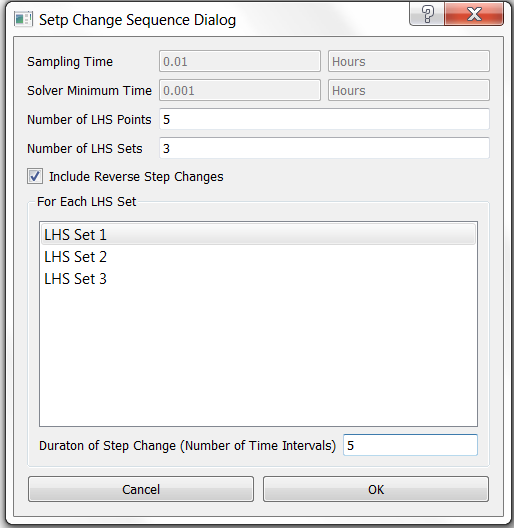
\includegraphics[scale=0.7]{Chapt_drm/figs/drm_training_sequence_dlg}
			\caption{Step Change Sequence Dialog Window}
			\label{fig.drm_training_sequence_dlg}
		\end{center}
	\end{figure}
	The sampling time interval and solver minimum time step are displayed in the first two read-only text boxes for reference.  The D-RM Builder uses the Latin Hypercube Sampling (LHS) method to fill the steady-state input space for input variables.  A sequence of step changes of the input variables, one at a time, is obtained by moving from one steady-state point to the next steady-state point in a set of LHS.  For each LHS point set, specify the number of steady-state points to be sampled.  For this example, enter 5 in the \textbf{\underline{Number of LHS Points}} text box.  Within each LHS point set, the holding time between the step changes or the duration of the step change is the same.  The durations for different LHS point sets should be varied such that different frequencies in a range can be excited.  Increasing the number of LHS point sets makes the step change sequence longer and the number of training data points larger, which generally leads to a more accurate D-RM.  It takes a longer CPU time to perform the ACM dynamic model simulation.  For this example, enter 3 in the \textbf{\underline{Number of LHS Sets}} text box and then press \textbf{\underline{Enter}}.  The number of items in the list box in the ``For Each LHS Set'' section is updated.  Three items are listed for this example.  Confirm that the \textbf{\underline{Include Reverse Step Changes}} check box is selected.  This means, the order of the step changes are reversed after the forward path from the first steady-state point to the last is completed, which makes the length of the step change sequence doubled.  For each LHS set, a holding duration is assigned.  The duration is measured as the number of sampling time intervals.  Click the ``LHS Set 1'' item in the ``For Each LHS Set'' list box and then enter 5 in the \textbf{\underline{Duration of Step Change}} text box.  Since the time interval is 0.01 hour in this case, the holding duration of 5 intervals corresponds to 0.05 hour of holding time.  Select the ``LHS Set 2'' item in the list box and then enter 10 in the \textbf{\underline{Duration of Step Change}} text box.  Select the ``LHS Set 3'' item in the list box and then enter 15 in the \textbf{\underline{Duration of Step Change}} text box.  It is recommended to enter different durations for different LHS sets such that it covers a range of frequencies of interest.  Click \textbf{\underline{OK}} to accept the inputs.  A confirmation message displays in the client area of the main window.
	\item Prepare an input change sequence for validation by issuing the \textbf{Setup $\rightarrow$ Prepare Validation Sequence} command or clicking the toolbar icon \includegraphics[scale=0.15]{Chapt_drm/figs/steps_valid}.  The ``Validation Sequence Dialog'' window displays as shown in Figure \ref{fig.drm_validation_sequence_dlg}.
	\begin{figure}[H]
		\begin{center}
			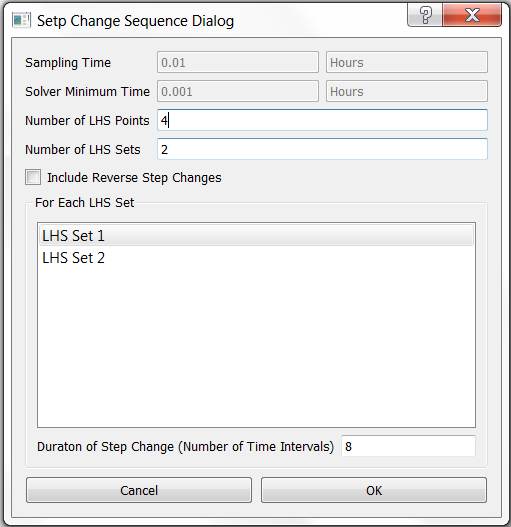
\includegraphics[scale=0.7]{Chapt_drm/figs/drm_validation_sequence_dlg}
			\caption{Validation Sequence Dialog Window}
			\label{fig.drm_validation_sequence_dlg}
		\end{center}
	\end{figure}
	The validation sequence is used as inputs for the high-fidelity model to simulate another set of response to validate the D-RM to be generated.  This command can be issued before or after the D-RM is generated.  In this example, create the step change sequence before the D-RM model is generated.  Enter 4 in the \textbf{\underline{Number of LHS Points}} text box.  Note: The number of LHS points is not necessarily the same as the value used for training.  Enter 2 in the \textbf{\underline{Number of LHS Sets}} text box.  Clear the \textbf{\underline{Include Reverse Step Change}s} check box.  Usually the sequence for validation is shorter than that for training to reduce the CPU time required to perform the high-fidelity model simulation.  Therefore, use fewer LHS sets and exclude the reverse step change.  Select the ``LHS Set 1'' item in the list box and then enter 8 for the duration of the first LHS set.  Then select the ``LHS Set 2'' item in the list box and then enter 12 for the duration of the second LHS set.  Note: The duration value for validation should be in the range of the training durations specified in the previous step.  Click \textbf{\underline{OK}} to accept the specifications.  A confirmation text message displays in the client area of the main window.
	\item Save the file by issuing the \textbf{File $\rightarrow$ Save} or \textbf{File $\rightarrow$ Save As} command or clicking the toolbar icon 
\includegraphics[scale=0.25]{Chapt_drm/figs/save}.  The ``Save D-RM Builder File'' dialog window displays.  Enter ``case1\_VdV'' in the file \textbf{\underline{Name}} text box and then click ``OK''.  A text file, ``case1\_VdV.drmb'', is written to the current working directory.  Note: The extension of the D-RM Builder case file is ``drmb''.  The file contains the user inputs that have been entered so far in JSON format.  If the user saves the case after completing the high-fidelity model simulations, the results of the simulations are also saved in the case file.  Likewise, if the user saves the case after a D-RM is generated, the data for the D-RM is also saved in the case file.  The D-RM Builder also keeps track of the status of the building process and knows what stage the user is in.  When the user opens an existing case file, the D-RM Builder brings the user to the stage that he or she left when the case was saved.
	\item Launch the ACM high-fidelity model simulation for training by issuing the \textbf{Build $\rightarrow$ Perform Training Simulation} command or clicking the toolbar icon \includegraphics[scale=0.15]{Chapt_drm/figs/run_train}.  This creates temporary files and a folder in the current working directory and brings up an ACM window.  The ACM simulation starts immediately.  The ACM iteration message can be viewed inside the ACM window if the ACM’s ``Simulation Message'' window is turned on.  The mouse icon is switched from normal (an arrow) to busy (rotating circle).  Wait without closing the ACM window.  After the high-fidelity model simulation is completed and the ACM window is closed, a message displays, confirming the successful completion of the high-fidelity model simulation.  The mouse icon becomes a normal arrow icon.  Note: The D-RM Builder calls ConsoleSinter.exe to perform dynamic ACM simulation and, therefore, the correct path for the ``SimSinter Home'' entry of the FOQUS \textbf{\underline{Settings}} needs to be configured before using the D-RM Builder.
	\item Launch the ACM high-fidelity model simulation for validation by issuing the \textbf{Build $\rightarrow$ Perform Validation Simulation} command or clicking the toolbar icon \includegraphics[scale=0.15]{Chapt_drm/figs/run_valid}.  Note: The background color of toolbar buttons for training are red and those for validation are green.  Wait until the ACM simulation is completed and the message confirming the successful completion of the simulation displays.
	\item Select DABNet as the D-RM model type by issuing the \textbf{Build $\rightarrow$ D-RM Model Type $\rightarrow$ DABNet} command and then confirming the ``DABNet'' pop-up submenu is checked as shown in Figure \ref{fig.drm_drm_type_dabnet}.
	\begin{figure}[H]
		\begin{center}
			\includegraphics[scale=0.7]{Chapt_drm/figs/drm_drm_type_dabnet}
			\caption{DABNet Submenu for Selecting a D-RM Model Type}
			\label{fig.drm_drm_type_dabnet}
		\end{center}
	\end{figure}
	Since the Decoupled A-B Net (DABNet) model is generated as the model type for this example, confirm the DABNet option is selected, which is the default option.
	\item Build the DABNet model by issuing the \textbf{Build $\rightarrow$ Generate Reduced Model} command or clicking the toolbar icon 
\includegraphics[scale=0.15]{Chapt_drm/figs/build_drm}.  The ``DABNet DRM Parameter Dialog'' window displays as shown in Figure \ref{fig.drm_dabnet_dlg}.
	\begin{figure}[H]
		\begin{center}
			\includegraphics[scale=0.7]{Chapt_drm/figs/drm_dabnet_dlg}
			\caption{DABNet DRM Parameter Dialog Window for VdV\_Reactor Model}
			\label{fig.drm_dabnet_dlg}
		\end{center}
	\end{figure}
	There is an ``Output Variable List'' list box and an ``Input Variable List'' list box in the upper left corner of the window.  Each output variable has its own DABNet model.  An array of the DABNet models is generated if multiple output variables exist.  In this case, there are two output variables and, therefore, two DABNet models are generated.  There are different options for building DABNet D-RM for each output variable.  In the ``For Each Output Variable'' section, the check box ``Linear Model'' is for the option to build linear D-RM using linear activation function in the ANN that maps the state-space variables to the output.  If this check box is selected, the \textbf{\underline{Number of Neurons in Hidden Layer}} will be automatically set to 1.  In this case, leave that check box cleared, indicating that a nonlinear D-RM is to be built. Leave the \textbf{\underline{Number of Neurons  in Hidden Layer}} to the default value of 10.  Select the default radio button of \textbf{\underline{Use Specified Pole Value}}.  The other three radio buttons are those for optimizing the pole values.  One major enhancement of D-RM Builder on the original DABNet model is the new formulation using two poles to handle a process with both fast and slow dynamics. If the double-pole option is needed for those two-time-scale systems, there are three options to optimize the pole values including both fast and slow poles, fast poles only, and slow poles only.  If the double-pole option is not selected, the user can select either the \textbf{\underline{Optimize Both Poles}} radio button or the \textbf{\underline{Optimize Fast Pole}} radio button to allow D-RM Builder to optimize the poles. For each input/output pair, the model parameters include the option to use double-pole formulation, time delay in terms of number of sampling time intervals, and the number of Laguerre states.  If double-pole option is selected, two sets of pole values and number of Laguerre states need to be specified, one for fast and the other for slow dynamics.  The D-RM Builder enables the user to define a fixed pole value for each input/output pair or to ask the software to optimize the pole values for the individual inputs.  Regarding the neural network training, there are two options available.  The first option, the default option, is the \textbf{\underline{Back Propagation}} (BP) method.  The second option is Interior Point Optimization (\textbf{\underline{IPOPT}}).  The D-RM building process involves the generation of discrete-time process matrices A and B based on Laguerre series and mapping the state space to the model outputs through a neural network, followed by a balanced realization of A and B matrices and mapping of balanced state space to the outputs through another neural network.  Therefore, two neural network trainings are required for each output variable.  Specify the training method and maximum number of training iterations for both Laguerre and balanced neural networks.  The initial weights of ANN connections can also slightly affect the results of balanced realization.  For this tutorial, use the default values for the model parameters and options by clicking \textbf{\underline{OK}} to accept the defaults.  The D-RM Builder starts the model generation process with multiple text messages displaying in the FOQUS console window.  Read the messages and pay attention to the relative training errors reported, especially for the balanced model.  A training error of less than 10$^{-4}$ (0.01\%) indicates a good selection of DABNet model parameters.  In this case the relative error of the DABNet model for the first output (Cb\_Product) is approximately 10$^{-5}$ (based on the balanced model) and that for the second output (Ca\_Product) is approximately $1.26\times10^{-5}$.  Note: The user may get different numbers depending on the version of ACM that is being used and the operating system the D-RM Builder is installed on.
	\item Save the case by issuing the \textbf{File $\rightarrow$ Save} command or clicking the toolbar icon 
\includegraphics[scale=0.25]{Chapt_drm/figs/save}.  Since the dynamic reduced model has been generated, it is time to save the case setup, high-fidelity model simulation results, and the data of the generated D-RM to the case file.
	\item To find how good the D-RM model prediction is compared to the high-fidelity model prediction, use the commands under the \textbf{\underline{Post-Process}} menu.  First confirm the ``Use Balanced Model for Prediction'' option under the \textbf{\underline{Post-Process}} menu is selected.  Usually this option is selected to examine the accuracy of the model.  If this option is cleared, the unbalanced Laguerre models are used for D-RM predictions.  Usually the unbalanced model predictions are not as accurate as the balanced model predictions, especially for the training sequence. 
	\item Examine the response for the training data.  To predict the training response using the generated D-RM, issue the \textbf{Post-Process $\rightarrow$ Predict Training Response} command or click the toolbar icon 
\includegraphics[scale=0.15]{Chapt_drm/figs/predict_train}.  The D-RM Builder calculates the response to the training sequence of the input changes based on the generated D-RM.  This command should be completed very quickly since the calculations for the D-RM based responses of the output variables are very fast.  A text message displays in the main window indicating the completion of the calculation.
	\item With both ACM and D-RM predictions for the response of the training sequence available, issue the \textbf{Post-Process $\rightarrow$ Plot Training Responses} command or click the toolbar icon 
\includegraphics[scale=0.15]{Chapt_drm/figs/plot_train} to visualize the results.  The ``Result Plotting Dialog'' window as shown in Figure \ref{fig.drm_plot_train_dlg} displays.
	\begin{figure}[H]
		\begin{center}
			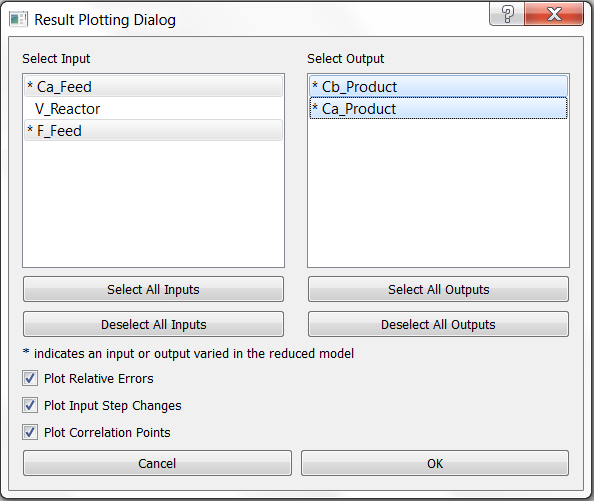
\includegraphics[scale=0.7]{Chapt_drm/figs/drm_plot_train_dlg}
			\caption{Result Plotting Dialog Window for VdV\_Reactor Model}
			\label{fig.drm_plot_train_dlg}
		\end{center}
	\end{figure}
	The ``Result Plotting Dialog'' window lists the input and output variables for the user to plot.  Note: The variable names listed with an asterisk (``*'') indicate the input or output variables that are varied (not fixed) in the reduced model.  Click the items in the list boxes to select and deselect the variables.  The four buttons below the two list boxes enable the user to select or deselect all of the input or output variables.  Here the user can select the first and the third input variables and the two output variables as shown in Figure \ref{fig.drm_plot_train_dlg}.  The D-RM Builder always plots the responses predicted by the generated D-RM and those by the ACM model in the first row of the figures.  The user can also plot the relative errors, input step changes, and correlation points by selecting the corresponding buttons in the lower part of the window.  Accept the defaults with all of the check boxes selected and then click \textbf{\underline{OK}}.  A Matplotlib window named ``Figure 1'' displays in a separate window as shown in Figure \ref{fig.drm_plot_train_fig}.
	\begin{figure}[H]
		\begin{center}
			\includegraphics[scale=0.7]{Chapt_drm/figs/drm_plot_train_fig}
			\caption{Plots of Input and Output Variables as Functions of Time for Training Data of VdV\_Reactor Model}
			\label{fig.drm_plot_train_fig}
		\end{center}
	\end{figure}
	Maximize the plot window to see the plots of the input and output variables clearly.  The plots in the top row are the curves of the output variables versus time.  If the user looks carefully, there are two curves plotted for each output variable.  The one in blue is the high-fidelity model (ACM model) simulation result and the other in red is the D-RM prediction.  The red curve seems to sit on the top of the blue one unless the user zooms in to a selected region.  The second row contains the normalized error plots showing the relative errors of the D-RM predictions compared to the ACM simulation results.  Notice that the relative errors are very small in this case, indicating that the generated D-RM fits the ACM model results very well.  The third row contains the plots of step changes of individual input variables, one input variable on each plot.  If the user looks carefully, the step changes of two inputs do not happen at the same time.  Actually the two inputs take turns to make step changes, one at a time.  The bottom row plots the points of the D-RM model predictions versus the ACM model predictions (plant data).  If a D-RM model prediction is exactly the same as the ACM model prediction, the point sits exactly on the 45 degree line if the scales of the two axes are identical.  The legends of the bottom row figures also show the R$^2$ values of the correlation.  As seen in Figure \ref{fig.drm_plot_train_fig}, the R$^2$ (coefficient of determination) values for the two outputs are very close to 1, indicating that the D-RM is quite accurate.  Note: R$^2$ is always less than 1.  Generally, the higher the R$^2$ value, the more accurate the generated D-RM.  Close the plot window by clicking the ``x'' at the upper right corner.  If needed, issue the \textbf{Post-Process $\rightarrow$ Plot Training Responses} command again with only one output variable selected at a time to visualize the plot in a single column.  Likewise, clear some of the check boxes in the ``Result Plotting Dialog'' window shown in Figure \ref{fig.drm_plot_train_dlg} to remove some of the rows of figures so the user can see the larger figures of interest.
	\item Examine the response for the validation data.  Usually the generated D-RM can predict the response of the training sequence very close to that from the high-fidelity model simulation since the reduced model is trained using the training data.  A good D-RM should also be able to predict the response of the validation data quite well.  To predict the validation response using the generated D-RM, issue the \textbf{Post-Process $\rightarrow$ Predict Validation Response} command or click the toolbar icon 
\includegraphics[scale=0.15]{Chapt_drm/figs/predict_valid}.
	\item Issue the \textbf{Post-Process $\rightarrow$ Plot Validation Responses} command or click the toolbar icon \includegraphics[scale=0.15]{Chapt_drm/figs/plot_valid}.  The ``Result Plotting Dialog'' window as shown in Figure \ref{fig.drm_plot_train_dlg} displays.  Select the first and the third input variables and the two output variables and click \textbf{\underline{O}K}.  A Matplotlib window named ``Figure 1'' displays in a separate window as shown in Figure \ref{fig.drm_plot_valid_fig}.
	\begin{figure}[H]
		\begin{center}
			\includegraphics[scale=0.7]{Chapt_drm/figs/drm_plot_valid_fig}
			\caption{Plots of Input and Output Data as Functions of Time for Validation Data}
			\label{fig.drm_plot_valid_fig}
		\end{center}
	\end{figure}
	Notice that the red curves are still on the top of the blue curves for both the Ca\_Product and Cb\_Product outputs, indicating a quite accurate D-RM generated by the D-RM Builder.  Close the plot window by clicking the ``x'' at the upper right corner.
	\item Save the file by clicking the toolbar icon 
\includegraphics[scale=0.25]{Chapt_drm/figs/save}.  The case file contains the data predicted by the D-RM generated for both the training and validation sequences.
	\item Perform the Uncertainty Quantification (UQ) analysis on the generated D-RM, using the ACM predictions as the plant data.  Note: The UQ commands are available only when the DABNet model option is selected.  For the UQ analysis, it is assumed that the process has certain noise in terms of standard deviation of state-space variables and the measurements of output variables also have noise in terms of standard deviations.  During the UQ analysis, the measured output values are obtained from the ACM prediction with the noise term added based on the standard deviation provided by the user.  To setup the noise levels of the state and output variables, issue the \textbf{UQ $\rightarrow$ Specify Noise} command or click the toolbar icon \includegraphics[scale=0.25]{Chapt_drm/figs/noise}.  The ``Noise Specification Dialog'' window as shown in Figure \ref{fig.drm_specify_noise_dlg} displays.
	\begin{figure}[H]
		\begin{center}
			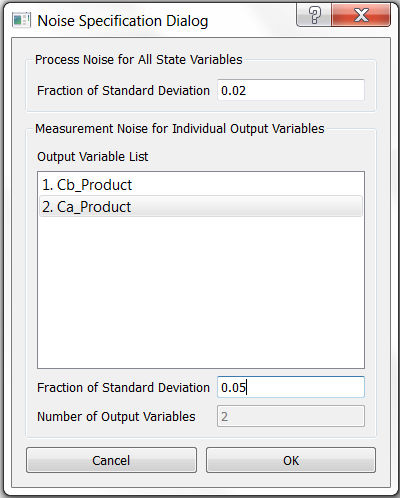
\includegraphics[scale=0.7]{Chapt_drm/figs/drm_specify_noise_dlg}
			\caption{Process and Measurement Noise Dialog Window for VdV\_Reactor Model}
			\label{fig.drm_specify_noise_dlg}
		\end{center}
	\end{figure} 
	Specify the noise as the fraction of the standard deviation of the state variables in the training sequence.  Note: Since the state variables could be either positive or negative in the normal operating conditions, the standard deviation of the state variables calculated in the training data is used as the basis for the noise level of the state variables.  In the current version, the ratio of the noise to the standard deviation of the state variable is assumed to be identical for any state variables, which is not necessarily true for a real-world process.  The identification of process noise has not been built in the current version of D-RM Builder.  The user can specify a single number for the noise level.  For this tutorial, use the default value of 0.02 in the \textbf{\underline{Fraction of Standard Deviation}} text box in the ``Process Noise for All State Variables'' section.  This means that the noise defined as the standard deviation of each state-space variable is 2\% of the standard deviation of the variable itself found in the training sequence.  The measurement noises can be specified separately, one for each output variable.  These noises are related to the sensitivity of the sensors and the electronics used to measure the output variables.  For this tutorial, select the first output variable ``1. Cb\_Product'' in the ``Output List'' and then enter 0.05 in the \textbf{\underline{Fraction of Standard Deviation}} text box in the ``Measurement Noise For Individual Output Variables" section.  Then, select the second variable ``2. Ca\_Product'' and then enter 0.05 as shown in Figure \ref{fig.drm_specify_noise_dlg}.  Click \textbf{\underline{OK}} to accept the noise specifications.
	\item Ask the D-RM Builder to perform the UQ analysis on the generated DABNet model following the validation step change sequence.  The algorithm of Unscented Kalman Filter (UKF) is used to predict the state variables step-by-step using the D-RM and to update the state and output variables using the measurement data, which is calculated by adding the random noise to the ACM predictions.  The mean values of the state and output variables are called ``filtered'' values, which are the weighted averages by considering both the D-RM predictions and measurements.  The Unscented Transform (UT) calculations are performed to calculate the means and covariances for the non-linear functions involved.  Multiple samples known as the sigma points around the means are used to evaluate the non-linear functions in the UT calculation.  The UT approach is proved in the literature to be much faster than Monte Carlo sampling with reasonable accuracy.  The covariance matrices are also updated step-by-step.  The elements in the covariance matrices tend to reach their asymptotic values after a certain period of time along the step change sequence.  To run the UQ analysis, issue the \textbf{UQ $\rightarrow$ Analyze} command or click the toolbar icon 
\includegraphics[scale=0.15]{Chapt_drm/figs/uq}.  The ``Result Plotting Dialog'' window as shown in Figure \ref{fig.drm_plot_train_dlg} displays, asking the user to specify the options for plotting the results of the UQ analysis.
	Since the volume of the reactor is constant, the user can select only the first and the third inputs in the ``Select Input Variables'' section on the window.  Select both output variables in the ``Select Output Variables'' section.  This time clear the \textbf{\underline{Plot Input Step Changes}} check box if the user is not interested in the input versus time plots.  Click \textbf{\underline{OK}}, the window closes, and the UQ calculation begins.  The calculation usually takes a while to complete since UKF algorithm is quite time consuming.  After the calculation is completed, the results are plotted in a pop-up window as show in Figure \ref{fig.drm_uq_fig}.
	\begin{figure}[H]
		\begin{center}
			\includegraphics[scale=0.7]{Chapt_drm/figs/drm_uq_fig}
			\caption{Plots Showing the Results of UQ Analysis for the Validation Sequence}
			\label{fig.drm_uq_fig}
		\end{center}
	\end{figure}
	Note: Due to the random nature of the noise added to the ACM prediction as the measurement data, the plotted figures could be slightly different from those shown in Figure \ref{fig.drm_uq_fig}.  Adjust the size of the plot window.  The first row of the plot window contains the two output variables (concentrations of Species A and B) as functions of time.  The black curves show the measured values which are calculated based on the ACM predictions and the randomly imposed measurement noise.  The red curves are the filtered mean output values.  The blue and green dotted curves show the error ranges (+/- the standard deviation from the calculated covariance matrix).  The relative errors and correlation plots are similar to those shown in Figure \ref{fig.drm_plot_valid_fig} except that both the D-RM and UKF results are plotted.  Since the generated D-RM is very accurate, the standard deviations of the output variables are dominated by the noise of the measurements, which is 5\% of the standard deviation of the output variable in the training data.
	\item Save the case by clicking the toolbar icon 
\includegraphics[scale=0.25]{Chapt_drm/figs/save}.  Export the covariance matrices at the end of the validation sequence by issuing the \textbf{File $\rightarrow$ Export $\rightarrow$ Covariance Matrices} command.  The ``Save Covariance Matrices'' dialog window displays.  Click \textbf{\underline{Save}} to accept the default name for the file.  The exported matrices are written in ``csv'' format.
	\item Export the generated D-RM to a MATLAB script file by issuing the \textbf{File $\rightarrow$ Export $\rightarrow$ D-RM As Matlab Script File} command.  The ``Save D-RM As Matlab Script'' dialog window displays.  Use the default file name ``case1\_VdV.m'' and then click \textbf{\underline{OK}} to save the D-RM to the ``case1\_VdV.m'' file.  This file is the main output file of the D-RM Builder and can be used by a MATLAB programmer for dynamic simulations.  The usage of this file is given in another tutorial in this manual.
	\item Save the log messages that have been displayed in the client area of the main window by selecting the \textbf{File $\rightarrow$ Export $\rightarrow$ Messages to Log File} command.  The ``Save Message Log'' dialog window displays.  Use the default file name ``case1\_VdV.log'' to save the log file.  The log file contains the information regarding the training errors and the optimized parameters during the reduced model building process, if applicable.  The information can be examined later when comparing to a new case with new user inputs.
	\item Save the actual input and output sequence data to a comma separated value (.csv) file by issuing the \textbf{File $\rightarrow$ Export $\rightarrow$ Training Data} command and the \textbf{File $\rightarrow$ Export $\rightarrow$ Validation Data} command for training data and validation data, respectively.  The data contains the step changes of inputs versus time and the responses predicted by the high-fidelity model.  If the D-RM predictions are available, they are also included in the exported file.
	\item Close the main window of the D-RM Builder by issuing the \textbf{File $\rightarrow$ Close} command or by clicking the toolbar icon \includegraphics[scale=0.25]{Chapt_drm/figs/close} to complete the model generation process.
\end{enumerate}

\subsection{Building Data-Driven D-RM using DABNet Framework and IPOPT-Based ANN Training}
In the previous example, the default back propagation (BP) method was used to train the neural networks inside the DABNet model.  The D-RM Builder provides an alternative method, the interior point optimization (IPOPT) method, to train the neural networks.  IPOPT is a general optimization algorithm to minimize an objective function as long as the code to evaluate the objective function, Jacobian matrix, and Hessian matrix is provided.  IPOPT is implemented in the D-RM Builder as an alternative to train neural networks in which the objective function is the sum of the errors squared at all discrete time points between the high-fidelity model prediction and the D-RM prediction.  Usually, the IPOPT method takes more CPU time than the default BP method.  Sometimes the IPOPT training method could minimize the training error (the objective function) to a lower value or generate a balanced model with fewer state-space variables than the back propagation method.  This tutorial demonstrates the usage of this option.

The Van-de-Vusse reactor example in the previous tutorial is modified in this tutorial. The following are the steps to build the D-RM using DABNet framework and IPOPT-based ANN training:
 
\begin{enumerate}
	\item Open Windows Explorer and browse to the FOQUS working directory and copy the \\``case1\_VdV.drmb'' file and rename it as ``case2\_VdV.drmb''.  This tutorial uses the case file ``case2\_VdV.drmb'' as the starting point and revises the D-RM training options.
	\item Start FOQUS.  The main window of the FOQUS displays.  Click the \textbf{\underline{DRM-Builder}} icon \includegraphics[scale=0.7]{Chapt_drm/figs/drm_icon_drmbuilder} and the embedded D-RM Builder frame displays as shown in Figure \ref{fig.drm_start}.
	\item Issue the \textbf{File $\rightarrow$ Open} command or click the toolbar icon 
\includegraphics[scale=0.15]{Chapt_drm/figs/open} to bring up the ``Open D-RM Builder File'' dialog. Browse to the FOQUS working directory, select the ``case2\_VdV.drmb'' file, and click the \textbf{\underline{Open}} button.
	\item Select the \textbf{Build $\rightarrow$ Generate Reduced Model} command or click the toolbar icon 
\includegraphics[scale=0.15]{Chapt_drm/figs/build_drm}.  The ``DABNet DRM Parameter Dialog'' window as shown in Figure \ref{fig.drm_dabnet_dlg} displays.  This time select the ``IPOPT'' option in both the ``Training Method For Laguerre Model Neural Network'' section and the ``Training Method For Balanced Model Neural Network'' section.  The IPOPT method can also be used to train the Laguerre model only and the BP method is used to train the balanced model.  Notice that the values in the text boxes of \textbf{\underline{Maximum Number of Training Iterations}} of both sections have changed.  These are the default values for the IPOPT training.  Since the IPOPT method is much slower than the back propagation method, the default maximum iteration numbers set by the D-RM Builder are smaller.  The user can increase the maximum iteration numbers.  For this tutorial, keep the default numbers.  Click \textbf{\underline{OK}} in the window to start the model generation process.  Text messages display in the FOQUS console window.  The mouse icon is switched from a normal (an arrow) icon to a busy (rotating circle) icon.  Be patient since the process to training the neural networks is slow.  Upon completion, a text message displays indicating that the D-RM has been generated and the mouse icon is switched back to the normal arrow icon.
	\item Use the commands under the \textbf{\underline{Post-Process}} menu to predict the training and validation responses using the new D-RM and visualize the results.  Notice that the training errors with the IPOPT option are slightly higher than those with the default back propagation option, probably because the maximum number of iterations in the IPOPT case are smaller.  However, this is not always the case.  For some non-linear cases, the IPOPT method could generate a better D-RM with smaller state-space size and higher accuracy.
	\item Perform UQ analysis by following the same procedure in the first tutorial to set the process and measurement noises and run the UQ analysis using the commands under the \textbf{\underline{UQ}} menu.
	\item Export the new D-RM to a file with an ``.m'' extension.  Save the case file and then close the D-RM Builder application.
\end{enumerate}

\subsection{Building Data-Driven D-RM using DABNet Framework with Pole Values Optimized}
Ideally, the pole value for each input/output pair in the DABNet model should match the time constant of the system for the output with respect to the input.  It is recommended by Sentoni et al. \cite{Sentoni_1998} that the pole value a should be set as:
$$a = 1-T_s/\tau$$
where $T_s$ is the sampling time interval set through the \textbf{Setup $\rightarrow$ Configure Input Variables} command and $\tau$ is the time constant of the output with respect to the input.  Note: The time constants are generally different for an output with respect to different inputs.  Therefore, different pole values should be used.  The exact value of the time constant for an input/output pair is hard to determine although a user can estimate that by running the high-fidelity model simulations.  Fortunately, the DABNet model is generally robust with respect to the user's selection of pole values.  A default value of 0.5 for each input/output pair could result in a D-RM with reasonable accuracy.  However, for some strongly non-linear systems, the accuracy of the generated D-RM is quite sensitive to the pole values especially when the selected sampling time interval does not match the time constant (the pole value $a$ calculated from the equation listed above is much higher or much lower than 0.5).  The D-RM Builder can optimize the pole values by minimizing the training error of the unbalanced Laguerre model.  Note: The optimization routine does not guarantee the global optimum and the user could provide the initial guess through the GUI of the D-RM Builder and the optimization is performed around the initial guess.  If the user has no idea about the reasonable initial guess, the default value of 0.5 is recommended.  This tutorial demonstrates the usage of the pole value optimization option.

To demonstrate the feature, an example named ``pH\_Neut'' is provided in a subfolder named ``pH'' in the D-RM Builder's example folder.  This example models the two-tank pH neutralization reactor described in \cite{Sentoni_1998}.  The default options are applied first to build a D-RM.  Then the user selects the pole value optimization option to see the improvement of the D-RM over the default option.  The DABNet model is still used as the D-RM model type.  The following are the steps to build a 
data-driven D-RM using DABNet framework with pole values optimized:

\begin{enumerate}
	\item Copy the ACM file of the pH\_Neut model ``pH\_Neut.acmf'' in ``C:\textbackslash Program Files (x86)\textbackslash foqus \textbackslash foqus\_2015.10.0\textbackslash examples\textbackslash DRMBuilder\textbackslash pH'' to the FOQUS working directory.  Confirm the user of the D-RM Builder has write-permissions to this folder.
	\item Launch SinterConfigGUI.  The GUI window as shown in Figure \ref{fig.sinter_gui_start} displays.
	\item Click the \textbf{\underline{Browse}} button and browse to the ``pH\_Neut.acmf'' file in the working directory.  Then click the \textbf{\underline{Open File and Configure Variables}} button.  It takes a few seconds for the SinterConfigGUI to display a ``SinterGonfigGUI Simulation Meta-Data'' window as shown in Figure \ref{fig.sinter_gui_meta_data_ph}.  An ACM window with pH\_Neut model inside also displays as shown in Figure \ref{fig.sinter_gui_acm_ph}.
	\begin{figure}[H]
		\begin{center}
			\includegraphics[scale=0.7]{Chapt_drm/figs/sinter_gui_meta_data_ph}
			\caption{Dialog Window for the Simulation Meta-Data of pH\_Neut Model}
			\label{fig.sinter_gui_meta_data_ph}
		\end{center}
	\end{figure}
	\begin{figure}[H]
		\begin{center}
			\includegraphics[scale=0.7]{Chapt_drm/figs/sinter_gui_acm_ph}
			\caption{ACM Window for pH\_Neut Model Displayed by SinterConfigGUI}
			\label{fig.sinter_gui_acm_ph}
		\end{center}
	\end{figure}
	\item Enter ``pH Neutralization Example'' in the \textbf{\underline{Title}} text box, ``My third DRMBuilder tutorial'' in the \textbf{\underline{Description}} text box, and the user's name in the \textbf{\underline{Author}} text box.  Then click the \textbf{\underline{Next}} button.  A ``SinterConfigGUI Variable Configuration Page'' window similar to Figure \ref{fig.sinter_gui_variable_config} displays.
	\item Enter ``$\sim$'' in the \textbf{\underline{Variable Search Pattern}} text box and click the \textbf{\underline{Search}} button.  All the variables in the pH\_Neut model are listed in the list box at the lower left corner of the window as shown in Figure \ref{fig.sinter_gui_search_ph}.
	\begin{figure}[H]
		\begin{center}
			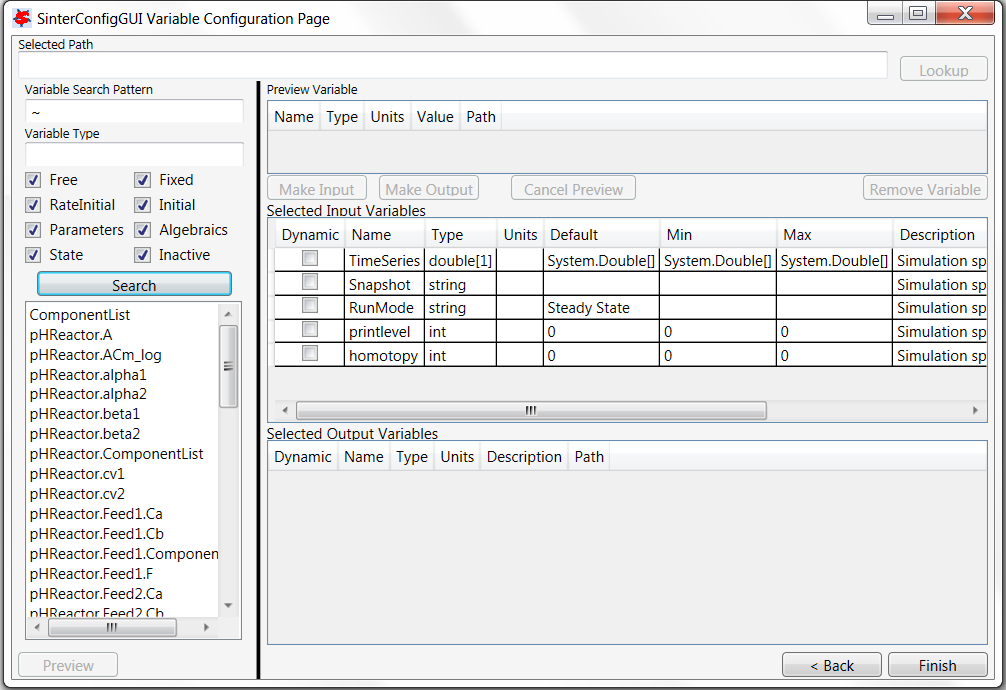
\includegraphics[scale=0.7]{Chapt_drm/figs/sinter_gui_search_ph}
			\caption{Variable List on Configuration Page of pH\_Neut Model}
			\label{fig.sinter_gui_search_ph}
		\end{center}
	\end{figure}
	\item Select the ``pHReactor.Feed1.F'' in the list box and click the \textbf{\underline{Lookup}} button at the upper right corner.  The variable is displayed in the ``Preview Variable'' section.  Click the \textbf{\underline{Make Input}} button and the variable is appended to the end of the ``Selected Input Variables'' table.  Change the name of the variable to ``F\_Feed1'' and select the checkbox in the \textbf{\underline{Dynamic}} column.  This makes the selected variable a dynamic input variable.
	\item Select the ``pHReactor.Feed2.F'' in the list box and repeat Step 6 to make it a dynamic input variable and change the name to ``F\_Feed2''.
	\item Select the ``pHReactor.Feed3.F'' in the list box and repeat Step 6 to make it a dynamic input variable and change the name to ``F\_Feed3''.
	\item Change the default value of the input variable named ``RunMode'' in the ``Selected Input Variables'' table from ``Steady State'' to ``Dynamic''.
	\item Select the ``pHReactor.pH'' in the list box and click the \textbf{\underline{Preview}} button.  Then click the \textbf{\underline{Make Output}} button and the variable is added to the ``Selected Output Variables'' table.  Change the name of the variable to ``pH\_Product'' and select the checkbox in the \textbf{\underline{Dynamic}} column.  This makes the selected variable a dynamic output variable.
	\item Select the ``pHReactor.Prod.Ca'' in the list box and repeat Step 10 to make it a dynamic output variable and change the name to ``Ca\_Product''.
	\item This concludes the configuration of ACM variables.  Figure \ref{fig.sinter_gui_final_ph} shows the SinterConfigGUI window after the configuration.  Click the \textbf{\underline{Next}} button at the lower right corner and a ``SinterConfigGUI Vector Default Initialization'' dialog window display as shown in Figure \ref{fig.sinter_gui_vector}.  Leave the default time series data unchanged.
	\begin{figure}[H]
		\begin{center}
			\includegraphics[scale=0.7]{Chapt_drm/figs/sinter_gui_final_ph}
			\caption{Configured Dynamic Variables of pH\_Neut Model by SinterConfigGUI}
			\label{fig.sinter_gui_final_ph}
		\end{center}
	\end{figure}
	\item Click the \textbf{\underline{Finish}} button to exit the ``SinterConfigGUI''.  A file named ``pH\_Neut.json'' is created in the working directory.  Close the ACM window.
	\item After the dynamic input and output variables are configured and the JSON file is created, start FOQUS.  The main window of the FOQUS displays.  Click the \textbf{\underline{Settings}} icon \includegraphics[scale=0.7]{Chapt_drm/figs/drm_icon_settings} and make sure the ``SimSinter Home'' is set to the full path of the folder where SinterConfigGUI.exe is located.  Click the \textbf{\underline{DRM-Builder}} icon \includegraphics[scale=0.7]{Chapt_drm/figs/drm_icon_drmbuilder} and the embedded D-RM Builder frame containing a blank project displays as shown in Figure \ref{fig.drm_start}.  
	\item To start the D-RM building process, a high-fidelity model (the pH\_Neut ACM model in this case) needs to be selected.  Issue \textbf{Setup $\rightarrow$ Choose High-Fidelity Model} command or click the toolbar icon \includegraphics[scale=0.12]{Chapt_drm/figs/aspen_tech}.  A ``SimSinter Configuration File'' window displays for file browsing and selecting.  Browse and select the ``pH\_Neut.json'' file created in Step 12.  This loads the configuration file into the D-RM Builder.  A text message confirming the file selection and loading displays in the client area of the D-RM Builder window.
	\item Configure the input variables. Navigate to the \textbf{Setup $\rightarrow$ Configure Input Variables} command or click the toolbar icon \includegraphics[scale=0.15]{Chapt_drm/figs/config_input}.  The ``Input Variable Dialog'' window displays as shown in Figure \ref{fig.drm_input_variable_dlg_ph}.
	\begin{figure}[H]
		\begin{center}
			\includegraphics[scale=0.7]{Chapt_drm/figs/drm_input_variable_dlg_ph}
			\caption{Input Variable Dialog Window for pH\_Neut Model}
			\label{fig.drm_input_variable_dlg_ph}
		\end{center}
	\end{figure}
	For this example, leave the default values of the lower and upper limits for the first and third variables unchanged.  Click the ``F\_Feed2'' item in the ``Input Variable List'' list box and then clear the \textbf{\underline{Varies With Time}} check box.  This makes the second input variable fixed (not changing with time).  Enter 0.005 in the \textbf{\underline{Sampling Time Interval}} text box.  Click \textbf{\underline{OK}} to accept the modifications and exit the window.
	\item Configure the output variables by issuing the \textbf{Setup $\rightarrow$ Configure Output Variables} command or clicking the toolbar icon \includegraphics[scale=0.2]{Chapt_drm/figs/config_output}.  The ``Output Variable Dialog'' window displays.  Accept the default options by clicking \textbf{\underline{OK}}.
	\item To prepare the training sequence, select the \textbf{Setup $\rightarrow$ Prepare Training Sequence} command or click the toolbar icon \includegraphics[scale=0.15]{Chapt_drm/figs/steps_train}.  The ``Step Change Sequence Dialog'' window displays.  For this example, enter 5 in the \textbf{\underline{Number of LHS Points}} text box and then enter 5 in the \textbf{\underline{Number of LHS Set}s} text box.  Five rows show in the ``For Each LHS Set'' list box.  Select the first row ``LHS Set 1'' item in the list box and then enter 5 in the \textbf{\underline{Duration of Step Change}} text box.  Select the second row ``LHS Set 2'' item in the list box and then enter 10 in the \textbf{\underline{Duration of Step Change}} text box.  Select the third row ``LHS Set 3'' item in the list box and then enter 15 in the \textbf{\underline{Duration of Step Change}} text box.  Select the fourth row ``LHS Set 4'' item in the list box and then enter 5 in the \textbf{\underline{Duration of Step Change}} text box.  Select the fifth row ``LHS Set 5'' item in the list box and then enter 10 in the \textbf{\underline{Duration of Step Change}} text box.  Confirm that the \textbf{\underline{Include Reverse Step Changes}} check box is selected.  Click \textbf{\underline{OK}} to accept the user inputs.
	\item Prepare an input change sequence for validation by issuing the \textbf{Setup $\rightarrow$ Prepare Validation Sequence} command or clicking the toolbar icon \includegraphics[scale=0.15]{Chapt_drm/figs/steps_valid}.  The ``Validation Sequence Dialog'' window displays.  Enter 5 in the \textbf{\underline{Number of LHS Points}} text box and then enter 2 in the \textbf{\underline{Number of LHS Sets}} text box.  Two rows show in the ``For Each LHS Set'' list box.  Select the first row ``LHS Set 1'' item in the list box and then enter 5 in the \textbf{\underline{Duration of Step Change}} text box.  Select the second row ``LHS Set 2'' item in the list box and then enter 10 in the \textbf{\underline{Duration of Step Change}} text box.  Click \textbf{\underline{OK}} to accept the change and then close the window.
	\item Save the file by issuing the \textbf{File $\rightarrow$ Save As} command.  The ``Save D-RM Builder File'' dialog window displays.  Enter ``case3\_pH\_Neut'' in the \textbf{\underline{File name}} text box and then click \textbf{\underline{OK}}.  A text file, ``case3\_pH\_Neut.drmb'', is written to the current working directory.
	\item Launch the ACM high-fidelity model simulation for training by issuing the \textbf{Build $\rightarrow$ Perform Training Simulation} command or clicking the toolbar icon \includegraphics[scale=0.15]{Chapt_drm/figs/run_train}.  This creates temporary files and a folder in the current working directory and displays an ACM window.  The ACM simulation starts immediately.  The ACM iteration message can be viewed inside the ACM window if the ACM’s ``Simulation Message'' window is activated.  The mouse icon is switched from normal (an arrow) to busy (rotating circle).  Wait without closing the ACM window.  After the high-fidelity model simulation is completed and the ACM window is closed, a message displays in the client window, confirming the successfully completion of the high-fidelity model simulation.  The mouse icon becomes a normal arrow icon.
	\item Launch the ACM high-fidelity model simulation for validation by issuing the \textbf{Build $\rightarrow$ Perform Validation Simulation} command or clicking the toolbar icon \includegraphics[scale=0.15]{Chapt_drm/figs/run_valid}.  Wait until the ACM simulation is completed and the message confirming the successful completion of the simulation displays.
	\item Select DABNet as the D-RM model type by issuing the \textbf{Build $\rightarrow$ D-RM Model Type $\rightarrow$ DABNet} command and then confirming the ``DABNet'' pop-up submenu is checked as shown in Figure \ref{fig.drm_drm_type_dabnet}.
	\item Build the DABNet model by issuing the \textbf{Build $\rightarrow$ Generate Reduced Model} command or clicking the toolbar icon \includegraphics[scale=0.15]{Chapt_drm/figs/build_drm}.  The ``DABNet DRM Parameter Dialog'' window displays as shown in Figure \ref{fig.drm_dabnet_dlg_ph}.  
	\begin{figure}[H]
		\begin{center}
			\includegraphics[scale=0.7]{Chapt_drm/figs/drm_dabnet_dlg_ph}
			\caption{DABNet Parameter Dialog Window for pH\_Neut Model}
			\label{fig.drm_dabnet_dlg_ph}
		\end{center}
	\end{figure}
	Click \textbf{\underline{OK}} in the window to accept all of the default options.  The default pole value is 0.5 for every input/output pair and the default neural network training method is back propagation.  Examine the text messages displayed in the console window of FOQUS to find that the relative error for training the balanced model of the first output variable is approximately 0.05475 while the error for the second variable is approximately 0.0017695.  These errors are quite high since the default pole values of 0.5 are not good for the dynamic process.  Note: The user may get different numbers depending on the version of ACM that is being used and the operating system the D-RM Builder is installed on.
	\item Save the case by issuing the \textbf{File $\rightarrow$ Save} command or clicking the toolbar icon \includegraphics[scale=0.25]{Chapt_drm/figs/save}.  Since the dynamic reduced model has been generated, it is time to save the case setup, high-fidelity model simulation results, and the data of the generated D-RM to the case file.
	\item To find how good the D-RM model prediction is compared to the high-fidelity model prediction, use the commands under the \textbf{\underline{Post-Process}} menu.  Confirm the ``Use Balanced Model for Prediction'' option under the \textbf{\underline{Post-Process}} menu is selected.
	\item Examine the response for the training data.  To predict the training response using the generated D-RM, issue the \textbf{Post-Process $\rightarrow$ Predict Training Response} command or click the toolbar icon \includegraphics[scale=0.15]{Chapt_drm/figs/predict_train}.
	\item Issue the \textbf{Post-Process $\rightarrow$ Plot Training Responses} command or click the toolbar icon \includegraphics[scale=0.15]{Chapt_drm/figs/plot_train} to visualize the results.  The ``Result Plotting Dialog'' window as shown in Figure \ref{fig.drm_plot_train_dlg_ph} displays.  Select the first and the third input variables (the variables that are marked with asterisks), both of the output variables, and then click \textbf{\underline{OK}}.  A Matplotlib window named ``Figure 1'' displays in a separate window as shown in Figure \ref{fig.drm_plot_train_fig_ph1}.
	\begin{figure}[H]
		\begin{center}
			\includegraphics[scale=0.7]{Chapt_drm/figs/drm_plot_train_dlg_ph}
			\caption{Result Plotting Dialog Window for pH\_Neut Model}
			\label{fig.drm_plot_train_dlg_ph}
		\end{center}
	\end{figure}
	\begin{figure}[H]
		\begin{center}
			\includegraphics[scale=0.7]{Chapt_drm/figs/drm_plot_train_fig_ph1}
			\caption{Plots Training Data of pH\_Neut Model with Default DABNet Parameters}
			\label{fig.drm_plot_train_fig_ph1}
		\end{center}
	\end{figure}
	Maximize the plot window to see the plots of the output variables clearly.  If the user looks carefully, there are two curves plotted for each output variable.  The one in blue is the high-fidelity model (ACM model) simulation result and the other in red is the D-RM prediction.  The user can find the mismatch between the two curves especially for the first variable (Ca\_Product) with a low R$^2$ value around 0.89.  The normalized error plots also show relative errors over 15\% in some regions.  Close the plot.  If needed, issue the \textbf{Post-Process $\rightarrow$ Plot/Compare Training Responses} command again with only one output variable selected at a time to visualize the plot in a higher resolution.
	\item Examine the response for the validation sequence.  To predict the validation response using the generated D-RM, issue the \textbf{Post-Process $\rightarrow$ Predict Validation Response} command or the toolbar icon \includegraphics[scale=0.15]{Chapt_drm/figs/predict_valid}.
	\item Issue the \textbf{Post-Process $\rightarrow$ Plot Validation Responses} command or click the toolbar icon \includegraphics[scale=0.15]{Chapt_drm/figs/plot_valid}.  The ``Result Plotting Dialog'' window as shown in Figure \ref{fig.drm_plot_train_dlg_ph} displays.  Select the first and the third input variables and all of the output variables and then click \textbf{\underline{OK}}.  A Matplotlib window named ``Figure 1'' displays in a separate window as shown in Figure \ref{fig.drm_plot_valid_fig_ph1}.  Notice that the relative errors of the D-RM predictions are quite high and the R$^2$ values are quite low, indicating an inaccurate D-RM generated by the D-RM Builder.  Click \textbf{\underline{OK}} to close the plot window.
	\begin{figure}[H]
		\begin{center}
			\includegraphics[scale=0.7]{Chapt_drm/figs/drm_plot_valid_fig_ph1}
			\caption{Plots Validation Data of pH\_Neut Model with Default DABNet Parameters}
			\label{fig.drm_plot_valid_fig_ph1}
		\end{center}
	\end{figure}
	\item Try to improve the D-RM accuracy by optimizing the pole values.  Build the D-RM again by issuing the \textbf{Build $\rightarrow$ Generate Reduced Model} command or clicking the toolbar icon \includegraphics[scale=0.15]{Chapt_drm/figs/build_drm}.  The ``DABNet DRM Parameter Dialog'' window displays.  This time, turn on the pole value optimization option.  In the ``Output Variable List'' list box, click the first output variable and then click the ``Optimize Fast Pole'' option in the ``For Each Output Variable'' section.  Meanwhile, enter 5 in the Number of Neurons in Hidden Layer edit box.  Click the second output variable and then click the ``Optimize Fast Pole'' option in the ``For Each Output Variable'' section.  Enter 5 in the \textbf{\underline{Number of Neurons in Hidden Laye}r} text box.  Select the first input variable in the ``Input Variable List'' list box and set the \textbf{\underline{Number of Laguerre States (Fast)}} text box to 7.  Repeat it for the second input variable.  In the ``Training Method for Laguerre Model Neural Network'' section, enter 7000 in the \textbf{\underline{Maximum Number of Training Iterations}} text box.  Click \textbf{\underline{OK}} to accept the option changes.  The D-RM Builder starts the D-RM generation process for both output variables, one at a time.  During the generation process, different pole values are tried to minimize the neural network training errors for the Laguerre models.  Text messages are displayed in FOQUS console window, including the optimized pole values and average training errors.  For example, the optimized pole values for the second output variable are 0.845556 and 0.864447 with respect to the first and second input variables.  The optimized pole values can also be displayed by issuing the \textbf{Build $\rightarrow$ Generate Reduced Model} command again. In the ``DABNet DRM Parameter Dialog'' window, select an output variable and then an input variable in the two list boxes and the corresponding pole value displays in the \textbf{\underline{Estimated Pole Value (Fast)}} text box.  Click \textbf{\underline{Cancel}} to exit the dialog window since the D-RM has been generated.
	\item Repeat Steps 27--30 to examine the predictions by the new D-RM.  Notice that the predicted responses by the new D-RM are in much better agreement with the responses predicted by the ACM model.  Figure \ref{fig.drm_plot_train_fig_ph2} shows the comparison of the training data. Notice that the R$^2$ values are very close to 1, indicating a good fit of the NABNet model to the ACM model. 
	\begin{figure}[H]
		\begin{center}
			\includegraphics[scale=0.7]{Chapt_drm/figs/drm_plot_train_fig_ph2}
			\caption{Plots Training Data of pH\_Neut Model with Optimized Pole Values}
			\label{fig.drm_plot_train_fig_ph2}
		\end{center}
	\end{figure}
	Figure \ref{fig.drm_plot_valid_fig_ph2} shows the comparison of the validation data.  Again the R$^2$ values for the validation data are much larger than those shown in 
	Figure \ref{fig.drm_plot_valid_fig_ph1}.  Therefore, the accuracy of the D-RM has been improved substantially after the pole value optimization.
	\begin{figure}[H]
		\begin{center}
			\includegraphics[scale=0.7]{Chapt_drm/figs/drm_plot_valid_fig_ph2}
			\caption{Plots Validation Data of pH\_Neut Model with Optimized Pole Values}
			\label{fig.drm_plot_valid_fig_ph2}
		\end{center}
	\end{figure}
	\item Perform the UQ analysis. Specify the process and measurement noise levels by issuing the \textbf{UQ $\rightarrow$ Specify Noise} command or clicking the toolbar icon \includegraphics[scale=0.25]{Chapt_drm/figs/noise}.  The ``Noise Specification Dialog'' window as shown in Figure \ref{fig.drm_specify_noise_dlg_ph} displays.
	\begin{figure}[H]
		\begin{center}
			\includegraphics[scale=0.7]{Chapt_drm/figs/drm_specify_noise_dlg_ph}
			\caption{Dialog Window for Specifying the Noise of pH\_Neut Model}
			\label{fig.drm_specify_noise_dlg_ph}
		\end{center}
	\end{figure}
	Set the \textbf{\underline{Fraction of Standard Deviation}} in the ``Process Noise for All State Variables'' section to 0.02.  In the section of ``Measurement Noise for Individual Output Variables'', click each output variable and set the \textbf{\underline{Fraction of Standard Deviation}} to 0.05.  Click \textbf{\underline{OK}} to accept the specified inputs.  Then launch the UQ calculation by issuing the \textbf{UQ $\rightarrow$ Calculate} command.  The ``Result Plotting Dialog'' window as shown in Figure \ref{fig.drm_plot_train_dlg_ph} displays.  Select the two input variables with ``*'' before the variable names and the two output variables.  This time clear the \textbf{\underline{Plot Input Step Changes}} check box and then click \textbf{\underline{OK}} to start the UQ calculation.  After the UQ calculation is completed, the results are plotted in a window as shown in Figure \ref{fig.drm_uq_fig_ph}.
	\begin{figure}[H]
		\begin{center}
			\includegraphics[scale=0.7]{Chapt_drm/figs/drm_uq_fig_ph}
			\caption{Plots of UQ Analysis for pH\_Neut Model}
			\label{fig.drm_uq_fig_ph}
		\end{center}
	\end{figure}
	\item Save the D-RM case, export the covariance matrices and the D-RM model, and then close the D-RM Builder case by issuing the corresponding commands under the \textbf{\underline{File}} menu.  Finally close the FOQUS main window without saving the FOQUS session.
\end{enumerate}

\subsection{Building Data-Driven D-RM using DABNet Framework with Ramp Changes to Replace Step Changes for Hard-to-Converge Stiff Models}
Depending on the dynamic system to be modeled, a high-fidelity model containing tens of thousands of DAEs could be hard to solve especially when those equations are very stiff.  For some complicated models, the change rates of certain input variables need to be kept low or the DAE solver fails to converge.  Typically, the D-RM Builder prepares a sequence of step changes of the input variables and performs the ACM simulation to calculate the output variables of the system responding to the step changes of the input variables.  A step change could be a big jump from one input condition to another, causing the DAE solver to fail to find a converged solution unless the internal time step for integration is extremely small.  To deal with this numerical problem, the big step change is approximated by a series of small steps at a constant ramp rate to reach the new input condition.  Therefore, the big step change is now replaced by a ramp change, which is implemented as multiple small step changes.  Note: A discrete-time 
D-RM has a fixed sampling time interval.  Those small step changes have to be completed to reach the desired input value within a fraction of the sampling time interval.  The maximum fraction permitted by the D-RM Builder is 0.5.  This option can be enabled through the GUI and the ramp rate specified.  This tutorial demonstrates the usage of this option.

To demonstrate the feature, an example is provided in a subfolder named ``BFB'' in the D-RM Builder's example folder.  This example models the sorbent-based two-bed bubbling fluidized bed (BFB) CO$_2$ adsorber-reactor system developed by a CCSI team.  This version of the BFB adsorber-reactor model contains over 20,000 DAEs.  The input variables include the flow rate, temperature, and composition of a feed flue gas stream.  The minimum integration time step is 0.001 second for the ACM solver while the sampling time interval for the D-RM is 0.1 second, which can be modified later.  Due to the complexity of the model, a step change of as low as 1 K in inlet flue gas temperature could cause the ACM model to fail to converge.  Likewise, a large step change in CO$_2$ mole fraction in the inlet flue gas could also cause the DAE solver to fail.  Therefore, use the ramp change option to approximate the step change.  The DABNet model is used as the D-RM type.  The pole value optimization option is used to generate the D-RM.  Note: A few hours are required to run the ACM simulations in this tutorial since the ACM model is complicated.  The following are the steps to build data-driven D-RM using DABNet framework with ramp changes to replace step changes for hard-to-converge stiff models:
%Please check formatting in #1 below. The file name goes beyond the right margin in the PDF. 
\begin{enumerate}
	\item Copy the ACM file of the BFB model ``BFB.acmf'' in \\``C:\textbackslash Program Files (x86)\textbackslash foqus\textbackslash foqus\_2015.10.0\textbackslash examples\textbackslash DRMBuilder\textbackslash BFB'' to the FOQUS working directory.  Confirm the user of the D-RM Builder has write-permissions to this folder.
	\item Launch SinterConfigGUI.  The GUI window as shown in Figure \ref{fig.sinter_gui_start} displays.
	\item Click the \textbf{\underline{Browse}} button and browse to the ``BFB.acmf'' file in the working directory.  Then click the \textbf{\underline{Open File and Configure Variables}} button.  It takes a few seconds for the SinterConfigGUI to display a ``SinterGonfigGUI Simulation Meta-Data'' window as shown in Figure \ref{fig.sinter_gui_meta_data_bfb}.  An ACM window with BFB model inside also displays as shown in Figure \ref{fig.sinter_gui_acm_bfb}.
	\begin{figure}[H]
		\begin{center}
			\includegraphics[scale=0.7]{Chapt_drm/figs/sinter_gui_meta_data_bfb}
			\caption{Dialog Window for the Simulation Meta-Data of BFB Model}
			\label{fig.sinter_gui_meta_data_bfb}
		\end{center}
	\end{figure}
	\begin{figure}[H]
		\begin{center}
			\includegraphics[scale=0.7]{Chapt_drm/figs/sinter_gui_acm_bfb}
			\caption{ACM Window for BFB Model Displayed by SinterConfigGUI}
			\label{fig.sinter_gui_acm_bfb}
		\end{center}
	\end{figure}
	\item Enter ``BFB Example'' in the \textbf{\underline{Title}} text box, ``My fourth DRMBuilder tutorial'' in the \textbf{\underline{Description}} text box, and the user's name in the \textbf{\underline{Author}} text box.  Then click the \textbf{\underline{Next}} button.  A ``SinterConfigGUI Variable Configuration Page'' window similar to Figure \ref{fig.sinter_gui_variable_config} displays.
	\item Enter ``ADSB.$\sim$'' in the \textbf{\underline{Variable Search Pattern}} text box and click the \textbf{\underline{Search}} button.  All the variables related to ADSB block are listed in the list box at the lower left corner of the window as shown in Figure \ref{fig.sinter_gui_search_bfb}.
	\begin{figure}[H]
		\begin{center}
			\includegraphics[scale=0.7]{Chapt_drm/figs/sinter_gui_search_bfb}
			\caption{Variable List on Configuration Page of BFB Model}
			\label{fig.sinter_gui_search_bfb}
		\end{center}
	\end{figure}
	\item Select the ``ADSB.GasIn.F'' in the list box and click the \textbf{\underline{Lookup}} button at the upper right corner.  The variable is displayed in the ``Preview Variable'' section.  Click the \textbf{\underline{Make Input}} button and the variable is appended to the end of the ``Selected Input Variables'' table.  Change the name of the variable to ``F\_GasIn'' and select the checkbox in the \textbf{\underline{Dynamic}} column.  This makes the selected variable a dynamic input variable.
	\item Select the ``ADSB.GasIn.T'' in the list box and repeat Step 6 to make it a dynamic input variable and change the name to ``T\_GasIn''.
	\item Enter ``zco2'' in the \textbf{\underline{Variable Search Pattern}} text box and click the \textbf{\underline{Search}} button.  Select the ``ZCO2'' in the list box and repeat Step 6 to make it a dynamic input variable and change the name to ``Z\_CO2''.
	\item Enter ``ADSA.$\sim$'' in the \textbf{\underline{Variable Search Pattern}} text box and click the \textbf{\underline{Search}} button.  All the variables related to ADSA block are listed in the list box at the lower left corner of the window. Find ``ADSA.SorbIn.Fm'' in the list and double-click the item.  The variable is shown in the ``Preview Variable'' table.  Click the \textbf{\underline{Make Input}} button and the variable is added to the ``Selected Input Variables'' table.  Make it a dynamic input variable and change the name to ``Fm\_SorbentIn''.
	\item Change the default value of the input variable named ``RunMode'' in the ``Selected Input Variables'' table from ``Steady State'' to ``Dynamic''.
	\item Enter ``co2removal'' in the \textbf{\underline{Variable Search Pattern}} text box and click the \textbf{\underline{Search}} button.  Then click the \textbf{\underline{Make Output}} button and the variable is added to the ``Selected Output Variables'' table.  Change the name of the variable to ``CO2\_Removal'' and select the checkbox in the \textbf{\underline{Dynamic}} column.  This makes the selected variable a dynamic output variable.
	\item Enter ``STACK.$\sim$'' in the \textbf{\underline{Variable Search Pattern}} text box and click the \textbf{\underline{Search}} button.  Select the ``STACK.Out2.F'' in the list box and repeat Step 10 to make it a dynamic output variable and change the name to ``F\_GasOut''.
	\item Select the ``STACK.Out2.T'' in the list box and repeat Step 10 to make it a dynamic output variable and change the name to ``T\_GasOut''.
	\item Select the ``STACK.Out2.Z(\text{"CO2"})'' in the list box and repeat Step 10 to make it a dynamic output variable and change the name to ``CO2\_GasOut''.
	\item This concludes the configuration of ACM variables.  Figure \ref{fig.sinter_gui_final_bfb} shows the SinterConfigGUI window after the configuration.  Click the \textbf{\underline{Next}} button at the lower right corner and a ``SinterConfigGUI Vector Default Initialization'' dialog window display as shown in Figure \ref{fig.sinter_gui_vector}.  Leave the default time series data unchanged.
	\begin{figure}[H]
		\begin{center}
			\includegraphics[scale=0.7]{Chapt_drm/figs/sinter_gui_final_bfb}
			\caption{Configured Dynamic Variables of BFB Model by SinterConfigGUI}
			\label{fig.sinter_gui_final_bfb}
		\end{center}
	\end{figure}
	\item Click the \textbf{\underline{Finish}} button to exit the ``SinterConfigGUI''.  A file named ``BFB.json'' is created in the working directory.  Close the ACM window.
	\item After the dynamic input and output variables are configured and the JSON file is created, start FOQUS.  The main window of the FOQUS displays.  Click the \textbf{\underline{Settings}} icon \includegraphics[scale=0.7]{Chapt_drm/figs/drm_icon_settings} and make sure the ``SimSinter Home'' is set to the full path of the folder where SinterConfigGUI.exe is located.  Click the \textbf{\underline{DRM-Builder}} icon \includegraphics[scale=0.7]{Chapt_drm/figs/drm_icon_drmbuilder} and the embedded D-RM Builder frame containing a blank project displays as shown in Figure \ref{fig.drm_start}.  
	\item To start the D-RM building process, a high-fidelity model (the BFB ACM model in this case) needs to be selected.  Issue \textbf{Setup $\rightarrow$ Choose High-Fidelity Model} command or click the toolbar icon \includegraphics[scale=0.12]{Chapt_drm/figs/aspen_tech}.  A ``SimSinter Configuration File'' window displays for file browsing and selecting.  Browse and select the ``BFB.json'' file.  This loads the configuration file into the D-RM Builder.  A text message confirming the file selection and loading displays in the client area of the D-RM Builder window.
	\item Configure the input variables.  Navigate to \textbf{Setup $\rightarrow$ Configure Input Variables} or click the toolbar icon \includegraphics[scale=0.15]{Chapt_drm/figs/config_input}.  The ``Input Variable Dialog'' window displays as shown in Figure \ref{fig.drm_input_variable_dlg_bfb}.
	\begin{figure}[H]
		\begin{center}
			\includegraphics[scale=0.7]{Chapt_drm/figs/drm_input_variable_dlg_bfb}
			\caption{Input Variable Dialog Window for BFB Model}
			\label{fig.drm_input_variable_dlg_bfb}
		\end{center}
	\end{figure}
	For this example, the first input variable ``Fm\_SorbentIn'' is kept as constant while the other three input variables are varied with time.  Click the first variable in the ``Input Variable List'' list box and clear the Varies With Time check box.  Change the \textbf{\underline{Sampling Time Interval}} from the 0.01 second to 0.2 second.  In the \textbf{\underline{Time Step During Ramp}} edit box, enter 0.005.  Next, enable the \textbf{\underline{Use Ramp To Replace Step Change}} option for the other three input variables in the ``Input Variable List'' list box.  Click the second item ``F\_GasIn'' in the list box and then select the \textbf{\underline{Use Ramp To Replace Step Change}} check box.  The \textbf{\underline{Ramp Rate}} text box is enabled.  Enter 13501 in the \textbf{\underline{Ramp Rate}} text box.  These are the user inputs for the flow rate of the feed flue gas stream.  Click the third item ``T\_GasIn'' in the list box and then select the \textbf{\underline{Use Ramp To Replace Step Change}} check box.  Enter 80 in the \textbf{\underline{Ramp Rate}} text box.  These are the user inputs for the temperature of the feed flue gas stream.  Click the fourth item ``Z\_CO2'' in the list box and then select the \textbf{\underline{Use Ramp To Replace Step Change}} check box.  Enter 0.264 in the \textbf{\underline{Ramp Rate}} text box.  These are the user inputs for the mole fraction of CO$_2$ in the feed flue gas stream.  Note: The ramp rate specified here for each input variable corresponds to the rate of change from the lower limit to the upper limit in half of the sampling time interval.   Click \textbf{\underline{OK}} to accept the modifications and exit the window.
	\item Configure the output variables by issuing the \textbf{Setup $\rightarrow$ Configure Output Variables} command or clicking the toolbar icon \includegraphics[scale=0.15]{Chapt_drm/figs/config_output}.  For this example, build the D-RM for all three output variables.  Clicking \textbf{\underline{OK}} to accept the default inputs.
	\item Prepare the training sequence, by selecting the \textbf{Setup $\rightarrow$ Prepare Training Sequence} command or clicking the toolbar icon \includegraphics[scale=0.15]{Chapt_drm/figs/steps_train}.  The ``Step Change Sequence Dialog'' window displays.  For this example, enter 5 in the \textbf{\underline{Number of LHS Points}} text box and then enter 4 in the \textbf\underline{{Number of LHS Sets}} text box.  Four rows show in the ``For Each LHS Set'' list box.  Select the first row ``LHS Set 1'' item in the list box and then enter 8 in the \textbf{\underline{Duration of Step Change}} text box.  Select the second row ``LHS Set 2'' item in the list box and then enter 10 in the \textbf{\underline{Duration of Step Change}} text box.  Select the third row ``LHS Set 3'' item in the list box and then enter 12 in the \textbf{\underline{Duration of Step Change}} text box.  Select the fourth row ``LHS Set 4'' item in the list box and then enter 14 in the \textbf{\underline{Duration of Step Change}} text box.  Confirm the \textbf{\underline{Include Reverse Step Changes}} check box is selected.  Click \textbf{\underline{OK}} to accept the user inputs.
	\item Prepare an input change sequence for validation by issuing the \textbf{Setup $\rightarrow$ Prepare Validation Sequence} command or clicking the toolbar icon \includegraphics[scale=0.15]{Chapt_drm/figs/steps_valid}.  The ``Step Change Sequence Dialog'' window displays.  Enter 5 in the \textbf{\underline{Number of LHS Points}} text box.  Leave all of the other entries in the window unchanged.  Click \textbf{\underline{OK}} to accept the change and then close the window.
	\item Save the file by issuing the \textbf{File $\rightarrow$ Save} command.  The ``Save As'' dialog window displays.  Enter ``case4\_BFB'' in the \textbf{\underline{File name}} text box and then click \textbf{\underline{OK}}.
	\item Launch the ACM high-fidelity model simulation for training by issuing the \textbf{Build $\rightarrow$ Perform Training Simulation} command or clicking the toolbar icon \includegraphics[scale=0.15]{Chapt_drm/figs/run_train}.  This creates temporary files and a folder in the current working directory and displays an ACM window.  The ACM simulation starts immediately.  The ACM iteration message can be viewed inside the ACM window if the ACM’s ``Simulation Message'' window is enabled.  The mouse icon is switched from normal (an arrow) to busy (rotating circle).  Wait for at least one hour without closing the ACM window.  After the high-fidelity model simulation is completed and the ACM window is closed, a message displays, confirming the successfully completion of the high-fidelity model simulation.  The mouse icon becomes a normal arrow icon.
	\item Launch the ACM high-fidelity model simulation for validation by issuing the \textbf{Build $\rightarrow$ Perform Validation Simulation} command or clicking the toolbar icon \includegraphics[scale=0.15]{Chapt_drm/figs/run_valid}.  Wait until the ACM simulation is completed and the message confirming the successful completion of the simulation displays.
	\item Select DABNet as the D-RM model type by issuing the \textbf{Build $\rightarrow$ D-RM Model Type $\rightarrow$ DABNet} command and then confirming the ``DABNet'' pop-up submenu is checked as shown in Figure \ref{fig.drm_drm_type_dabnet}.
	\item Build the DABNet model by issuing the \textbf{Build $\rightarrow$ Generate Reduced Model} command or clicking the toolbar icon \includegraphics[scale=0.15]{Chapt_drm/figs/build_drm}.  The ``DABNet DRM Parameter Dialog'' window displays.  Enable the pole value optimization option for each output variable.  Select an output variable in the \textbf{\underline{Output Variable List}} box and then click either the \textbf{\underline{Optimize Both Poles}} or the \textbf{\underline{Optimize Fast Pole}} radio button in the ``For Each Output Variable'' section.  Repeat this for all the output variables.  Click \textbf{\underline{OK}} in the window to accept all of the modifications.  The D-RM Builder starts to train the DABNet models with the pole values optimized.  It could take quite a while to complete the training and optimization process since the D-RM contains three input variables and three output variables.  The mouse icon changes to the busy (rotating circle) icon until the model generation process is completed.
	\item Save the case by issuing the \textbf{File $\rightarrow$ Save} command or clicking the toolbar icon \includegraphics[scale=0.25]{Chapt_drm/figs/save}.  Since the dynamic reduced model has been generated, it is time to save the case setup, high-fidelity model simulation results, and the data of the generated D-RM to the case file.
	\item To find how good the D-RM model prediction is compared to the high-fidelity model prediction, use the commands under the \textbf{\underline{Post-Process}} menu.  Confirm the ``Use Balanced Model for Prediction'' option under the \textbf{\underline{Post-Process}} menu is selected. 
	\item Examine the response for the training data.  To predict the training response using the generated D-RM, issue the \textbf{Post-Process $\rightarrow$ Predict Training Response} command.
	\item Issue the \textbf{Post-Process $\rightarrow$ Plot Training Responses} command.  The ``Result Plotting Dialog'' window as shown in Figure \ref{fig.drm_plot_train_dlg_bfb} displays.
	\begin{figure}[H]
		\begin{center}
			\includegraphics[scale=0.7]{Chapt_drm/figs/drm_plot_train_dlg_bfb}
			\caption{Dialog Window for Plotting Training Data of BFB Model}
			\label{fig.drm_plot_train_dlg_bfb}
		\end{center}
	\end{figure}
	Select the input variable ``F\_GasIn'' in the ``Select Input Variables'' list, select the output variable ``CO2\_Removal'' in the ``Select Output Variables'' list, and then click \textbf{\underline{OK}}.  A plot window as show in Figure \ref{fig.drm_plot_train_dlg_bfb} displays.
	\begin{figure}[H]
		\begin{center}
			\includegraphics[scale=0.7]{Chapt_drm/figs/drm_plot_train_fig_bfb}
			\caption{Response of Training Data of BFB Model}
			\label{fig.drm_plot_train_fig_bfb}
		\end{center}
	\end{figure}
	Maximize the plot window to see the plots of the output variables clearly.  If the user looks carefully, there are two curves plotted for each output variable.  The one in blue is the high-fidelity model (ACM model) simulation result and the other in red is the D-RM prediction.  Close the plot window after examining the results for the training sequence.  If needed, issue the \textbf{Post-Process $\rightarrow$ Plot Training Responses} command again to view the plot for other output variables.
	\item Examine the response for the validation data.  To predict the validation response using the generated D-RM, issue the \textbf{Post-Process $\rightarrow$ Predict Validation Response} command or click the toolbar icon \includegraphics[scale=0.15]{Chapt_drm/figs/predict_valid}.
	\item Issue the \textbf{Post-Process $\rightarrow$ Plot Validation Responses} command or click on the toolbar \includegraphics[scale=0.15]{Chapt_drm/figs/plot_valid}.  The ``Result Plotting Dialog'' window as shown in Figure \ref{fig.drm_plot_train_dlg_bfb} displays.  Select one or a few input variables and one or a few output variables and then click \textbf{\underline{OK}}.  A plot window displays.  Close the plot window after examining the plots.
	\item Save the D-RM case, export the D-RM model, and close the D-RM Builder window by issuing the corresponding commands under the \textbf{\underline{File}} menu.  Finally, close the FOQUS main window without saving the FOQUS session file.
\end{enumerate}

\subsection{Building Data-Driven D-RM using DABNet for Two-Time-Scale Process}
The previous tutorial demonstrates the ability of DABNet D-RM to model the fast dynamics of CCSI's BFB adsorber-reactor since the sampling time interval of 0.2 second is short and so is the duration between two step changes.  With short durations, the process is always in transient mode without reaching steady-state conditions.  As a matter of fact, the BFB adsorber-reactor is a system that has two time scales, a fast one due to fast fluid dynamics and a slow one due to the reactivity of solid sorbent.  This tutorial demonstrates how to model a two-time-scale process using double-pole DABNet D-RM.

This tutorial uses the same BFB adsorber-reactor ACM model in the previous tutorial and the same JSON file configured by SinterConfigGUI.  The following are the steps to build the D-RM.

\begin{enumerate}
	\item Make sure the ``BFB.json'' file created in the previous tutorial is in the FOQUS working directory.  Start FOQUS.  The main window of the FOQUS displays.
	\item Configure the input variables.  Navigate to \textbf{Setup $\rightarrow$ Configure Input Variables} or click the toolbar icon \includegraphics[scale=0.15]{Chapt_drm/figs/config_input}.  The ``Input Variable Dialog'' window as shown in Figure \ref{fig.drm_input_variable_dlg_bfb} displays.
	\item With the first input variable ``Fm\_SorbentIn'' selected in the list box, click the \textbf{\underline{Down}} arrow button.  The variable becomes the second item in the list box.
	\item In this tutorial, the feed flue gas temperature and the mole fraction in the flue gas are kept constant.  Select the ``T\_GasIn'' in the list box and make sure the \textbf{\underline{Varies With Time}} check box is cleared.  Repeat for the ``Z\_CO2'' input variable.  Since flue gas temperature and mole fraction are kept constant, the \textbf{\underline{Use Ramp to Replace Step Change}} check box is cleared for the first two input variables that vary with time.  Enter 1 in the \textbf{\underline{Sampling Time Interval}} text box.  Accept all other default inputs and click \textbf{\underline{OK}}.
	\item Configure the output variables by issuing the \textbf{Setup $\rightarrow$ Configure Output Variables} command or clicking the toolbar icon \includegraphics[scale=0.15]{Chapt_drm/figs/config_output}.  For this example, build the D-RM for ``CO2\_Removal'' only.  Select ``F\_GasOut'' and clear the \textbf{\underline{Varies With Time}} check box.  Repeat for the output variable ``T\_GasOut''. Click \textbf{\underline{OK}} to accept the changes.
	\item Prepare the training sequence, by selecting the \textbf{Setup $\rightarrow$ Prepare Training Sequence} command or clicking the toolbar icon \includegraphics[scale=0.15]{Chapt_drm/figs/steps_train}.  The ``Step Change Sequence Dialog'' window displays.  For this example, enter 5 in the \textbf{\underline{Number of LHS Points}} text box and then enter 4 in the \textbf{\underline{Number of LHS Sets}} text box.  Four rows display in the ``For Each LHS Set'' list box.  Select the first row ``LHS Set 1'' item in the list box and then enter 20 in the \textbf{\underline{Duration of Step Change}} text box.  Select the second row ``LHS Set 2'' item in the list box and then enter 40 in the \textbf{\underline{Duration of Step Change}} text box.  Select the third row ``LHS Set 3'' item in the list box and then enter 60 in the \textbf{\underline{Duration of Step Change}} text box.  Select the fourth row ``LHS Set 4'' item in the list box and then enter 80 in the \textbf{\underline{Duration of Step Change}} text box.  Confirm the Include Reverse Step Changes check box is selected.  Click \textbf{\underline{OK}} to accept the user inputs.
	\item Prepare an input change sequence for validation by issuing the \textbf{Setup $\rightarrow$ Prepare Validation Sequence} command or clicking the toolbar icon \includegraphics[scale=0.15]{Chapt_drm/figs/steps_valid}.  The ``Step Change Sequence Dialog'' window displays.  Enter 5 in the \textbf{\underline{Number of LHS Points}} text box and then enter 2 in the \textbf{\underline{Number of LHS Sets}} text box.  Select the first row ``LHS Set 1'' item in the list box and then enter 20 in the \textbf{\underline{Duration of Step Change}} text box.  Select the second row ``LHS Set 2'' item in the list box and then enter 40 in the \textbf{\underline{Duration of Step Change}} text box.  Click \textbf{\underline{OK}} to accept the change and then close the window.
	\item Save the file by issuing the \textbf{File $\rightarrow$ Save} command.  The ``Save As'' dialog window displays.  Enter ``case5\_BFB'' in the \textbf{\underline{File name}} text box and then click \textbf{\underline{OK}}.
	\item Launch the ACM high-fidelity model simulation for training by issuing the \textbf{Build $\rightarrow$ Perform Training Simulation} command or clicking the toolbar icon \includegraphics[scale=0.15]{Chapt_drm/figs/run_train}.  This creates temporary files and a folder in the current working directory and displays an ACM window.  The ACM simulation starts immediately.  The ACM iteration message can be viewed inside the ACM window if the ACM’s ``Simulation Message'' window is enabled.  The mouse icon is switched from normal (an arrow) to busy (rotating circle).  Wait for at least one hour without closing the ACM window.  After the high-fidelity model simulation is completed and the ACM window is closed, a message displays, confirming the successfully completion of the high-fidelity model simulation.  The mouse icon becomes a normal arrow icon.
	\item Launch the ACM high-fidelity model simulation for validation by issuing the \textbf{Build $\rightarrow$ Perform Validation Simulation} command or clicking the toolbar icon \includegraphics[scale=0.15]{Chapt_drm/figs/run_valid}.  Wait until the ACM simulation is completed and the message confirming the successful completion of the simulation displays.
	\item Select DABNet as the D-RM model type by issuing the \textbf{Build $\rightarrow$ D-RM Model Type $\rightarrow$ DABNet} command and then confirming the ``DABNet'' pop-up submenu is checked as shown in Figure \ref{fig.drm_drm_type_dabnet}.
	\item Build the DABNet model by issuing the \textbf{Build $\rightarrow$ Generate Reduced Model} command or clicking the toolbar icon \includegraphics[scale=0.15]{Chapt_drm/figs/build_drm}.  The ``DABNet DRM Parameter Dialog'' window displays.  Select the only output variable ``CO2\_Removal'' in the ``Output Variable List'' box.  Enter 2 in the \textbf{\underline{Number of Neurons in Hidden Layer}} text box.  Click the \textbf{\underline{Optimize Both Poles}} radio button in the ``For Each Output Variable'' section.  Select the \textbf{\underline{Use Two Poles (Fast and Slow)}} check box for each input variable.  Leave the default value of 0.5 for the fast pole unchanged.  Enter 0.99 for the slow pole for each input variable as shown in Figure \ref{fig.drm_dabnet_dlg_bfb2}.  Click \textbf{\underline{OK}}  to accept all of the modifications.  The D-RM Builder starts to train the DABNet models with the pole values optimized.  It could take quite a while to complete the training and optimization process since the D-RM contains three input variables.  The mouse icon changes to the busy (rotating circle) icon until the model generation process is completed.
	\begin{figure}[H]
		\begin{center}
			\includegraphics[scale=0.7]{Chapt_drm/figs/drm_dabnet_dlg_bfb2}
			\caption{DABNet Parameter Dialog Window for Two-Time-Scale BFB Model}
			\label{fig.drm_dabnet_dlg_bfb2}
		\end{center}
	\end{figure}
	\item Save the case by issuing the \textbf{File $\rightarrow$ Save} command or clicking the toolbar icon \includegraphics[scale=0.25]{Chapt_drm/figs/save}.  Since the dynamic reduced model has been generated, it is time to save the case setup, high-fidelity model simulation results, and the data of the generated D-RM to the case file.
	\item To find how good the D-RM model prediction is compared to the high-fidelity model prediction, use the commands under the \textbf{\underline{Post-Process}} menu.  Confirm the ``Use Balanced Model for Prediction'' option under the \textbf{\underline{Post-Process}} menu is selected. 
	\item Examine the response for the training data.  To predict the training response using the generated D-RM, issue the \textbf{Post-Process $\rightarrow$ Predict Training Response} command.
	\item Issue the \textbf{Post-Process $\rightarrow$ Plot Training Responses} command.  The ``Result Plotting Dialog'' window as shown in Figure \ref{fig.drm_plot_train_dlg_bfb2} displays.
	\begin{figure}[H]
		\begin{center}
			\includegraphics[scale=0.7]{Chapt_drm/figs/drm_plot_train_dlg_bfb2}
			\caption{Dialog Window for Plotting Training Data of Two-Time-Scale BFB Model}
			\label{fig.drm_plot_train_dlg_bfb2}
		\end{center}
	\end{figure}
	Select the input variable ``F\_GasIn'' in the ``Select Input Variables'' list, select the output variable ``CO2\_Removal'' in the ``Select Output Variables'' list, and then click \textbf{\underline{OK}}.  A plot window as show in Figure \ref{fig.drm_plot_train_dlg_bfb2} displays.
	\begin{figure}[H]
		\begin{center}
			\includegraphics[scale=0.7]{Chapt_drm/figs/drm_plot_train_fig_bfb2}
			\caption{Response of Training Data of Two-Time-Scale BFB Model}
			\label{fig.drm_plot_train_fig_bfb2}
		\end{center}
	\end{figure}
	Maximize the plot window to see the plots of the output variables clearly.  If the user looks carefully, there are two curves plotted for each output variable.  The one in blue is the high-fidelity model (ACM model) simulation result and the other in red is the D-RM prediction.  It can be seen from the figure that there is a quick response in a few seconds followed by a slow response whenever there is an input step change.  Close the plot window after examining the results for the training sequence.  If needed, issue the \textbf{Post-Process $\rightarrow$ Plot Training Responses} command again to view the plot for other output variables.
	\item Examine the response for the validation data.  To predict the validation response using the generated D-RM, issue the \textbf{Post-Process $\rightarrow$ Predict Validation Response} command or click the toolbar icon \includegraphics[scale=0.15]{Chapt_drm/figs/predict_valid}.
	\item Issue the \textbf{Post-Process $\rightarrow$ Plot Validation Responses} command or click on the toolbar \includegraphics[scale=0.15]{Chapt_drm/figs/plot_valid}.  The ``Result Plotting Dialog'' window as shown in Figure \ref{fig.drm_plot_train_dlg_bfb2} displays.  Select one or a few input variables and one or a few output variables and then click \textbf{\underline{OK}}.  A plot window displays.  Close the plot window after examining the plots.
	\item Save the D-RM case, export the D-RM model, and close the D-RM Builder window by issuing the corresponding commands under the \textbf{\underline{File}} menu.  Finally, close the FOQUS main window without saving the FOQUS session file.
\end{enumerate}

\subsection{Building Data-Driven D-RM using NARMA Framework}
The Nonlinear Autoregressive Moving Average (NARMA) model is another type of D-RM implemented in the D-RM Builder.  This is also a discrete-time plant identification model \cite{Narendra_1997}.  This model is simpler than the DABNet model in terms of model formulation.  In this model, the predicted value of an output variable at the next future time step is a function of the current and past values of the input and output variables.  The functional relationship is modeled by an artificial feed-forward neural network with a single hidden layer.  No internal state-space variables are included in this model.  Therefore, this model is simply an input/output mapping.  The user inputs for the model generation include only the number of neurons in the hidden layer of the neural network and the number of discrete historical time steps.

The Van-de-Vusse reactor model created in the first tutorial of this manual is used as the 
high-fidelity model for this tutorial.  Since the high-fidelity model simulations have been performed in the first tutorial, those results saved in the case file ``case1\_VdV.json'' can be used to build the NARMA model.  The following are the steps to generate the NARMA-based D-RM.

\begin{enumerate}
	\item Open Windows Explorer and browse to the FOQUS working directory and copy the ``case1\_VdV.json'' file and rename it as ``case5\_VdV.json''.  This tutorial uses the case file ``case5\_VdV.json'' as the starting point and revise the D-RM training options.
	\item Start FOQUS.  The main window of the FOQUS displays.  Click the \textbf{\underline{DRM-Builder}} icon \includegraphics[scale=0.7]{Chapt_drm/figs/drm_icon_drmbuilder} and the embedded D-RM Builder frame displays as shown in Figure \ref{fig.drm_start}.
	\item Issue the \textbf{File $\rightarrow$ Open} command or click the toolbar icon \includegraphics[scale=0.15]{Chapt_drm/figs/open} to display the ``Open D-RM Builder File'' dialog. Browse to the FOQUS working directory, select the ``case5\_VdV.json'' file, and click the \textbf{\underline{Open}} button.
	\item Select the \textbf{Build $\rightarrow$ D-RM Model Type $\rightarrow$ NARMA} command.  This switches the D-RM model type from DABNet to NARMA.
	\item Select the \textbf{Build $\rightarrow$ Generate Reduced Model} command or click the toolbar icon \includegraphics[scale=0.15]{Chapt_drm/figs/build_drm}.  The ``NARMA DRM Parameter Dialog'' window as shown in Figure \ref{fig.drm_narma_dlg} displays.
	\begin{figure}[H]
		\begin{center}
			\includegraphics[scale=0.7]{Chapt_drm/figs/drm_narma_dlg}
			\caption{Dialog Window for Building a NARMA Model}
			\label{fig.drm_narma_dlg}
		\end{center}
	\end{figure}
	Notice that the dialog window is different from the window for the DABNet model.  The value in the \textbf{\underline{Number of Discrete History Data}} text box indicates the number of historical data points (for both the input and output types of variables) to be used in the NARMA model.  If this number is 1, only the data at the current time is used to predict the outputs of the next time step.  Typically, this number should be either 2 or 3.  Enter the number of neurons in the hidden layer in the second text box.  This value is generally related to the total number of the input and output variables.  A large number should be used if the numbers of input and output variables are large.  Too large a number of hidden neurons could possibly over-fit the training data which could cause the accuracy for the validation data to decrease.  The user can manually modify this D-RM parameter to obtain the best fit for the validation data.  In the current version of the D-RM Builder, no procedure has been implemented to optimize the number of neurons in the hidden layer.  Enter the maximum number of back propagation iterations in the third text box.  Note: For the NARMA model, back propagation algorithm for the neural network training should work quite well and the IPOPT algorithm is not provided as an option.  For this example, accept the default values and then click \textbf{\underline{OK}}.  The training process starts immediately.  The mouse icon is switched to a busy (rotating circle) icon until the training process is completed.
	\item Before predicting the responses for the training and validation sequences using the generated D-RM, select where to get the historical output data.  Since the NARMA model requires the historical output data as inputs to the neural network, the user can either use the “true” data, which are the high-fidelity model simulation results in this case, or the output data predicted by the NARMA model itself from previous steps.  The D-RM Builder enables the user to use one of the two options.  Try both options in this tutorial.  First navigate to \textbf{Post-Process $\rightarrow$ Use High-Fidelity Model History For Prediction} and then confirm this option is selected.  This option makes the D-RM Builder use the high-fidelity model simulation results in the current and previous time steps to predict the response of a future time step.
	\item Use the commands under the \textbf{\underline{Post-Process}} menu to predict the training and validation responses using the NARMA D-RM that has just been generated and then visualize the results.  For example, click \includegraphics[scale=0.15]{Chapt_drm/figs/predict_valid} followed by \includegraphics[scale=0.15]{Chapt_drm/figs/plot_valid} on the toolbar to plot the predictions for the validation sequences.  Figure \ref{fig.drm_narma_fig} shows the plots of the validation data.
	\begin{figure}[H]
		\begin{center}
			\includegraphics[scale=0.7]{Chapt_drm/figs/drm_narma_fig}
			\caption{Predictions of Validation Sequence Using High-Fidelity Model History Data}
			\label{fig.drm_narma_fig}
		\end{center}
	\end{figure}
	Notice that when the ``true'' output values of the current and previous time steps are used, the predicted responses by the NARMA model are in good agreement with the 
	high-fidelity model predictions.  This means the NARMA model is capable of predicting short-term future responses given the accurate values of the output variables at the moment and in the near history.
	\item To try the other prediction option, navigate to \textbf{Post-Process $\rightarrow$ Use High-Fidelity Model History For Prediction} and then confirm it is cleared.  This makes the D-RM Builder use the current and previous output values predicted by D-RM itself to predict the output values for the next time step.
	\item Repeat the commands in Step 7 by clicking the \includegraphics[scale=0.15]{Chapt_drm/figs/predict_valid} icon followed by the \includegraphics[scale=0.15]{Chapt_drm/figs/plot_valid} icon on the toolbar.  Figure \ref{fig.drm_narma_fig_drm_only} shows the plots of the validation sequence.
	\begin{figure}[H]
		\begin{center}
			\includegraphics[scale=0.7]{Chapt_drm/figs/drm_narma_fig_drm_only}
			\caption{Predictions for Validation Sequence Using D-RM Predicted History Data}
			\label{fig.drm_narma_fig_drm_only}
		\end{center}
	\end{figure}
	It can be seen that the D-RM predictions are very different from the high-fidelity model predictions except in the first few time steps.  Oscillations are found from the D-RM predictions.  This means the NARMA model is not good for long-term prediction without using the measured plant output data.  The DABNet models, on the other hand, are capable of predicting quite accurately long-term responses without the need for the measured output data.  Therefore, DABNet is more suitable for model predictive control in which the maneuver through control variables is optimized on a quite long time horizon.
	\item Export the NARMA-based D-RM to a file with an “.m” extension.  Note: When \textbf{Build $\rightarrow$ D-RM Model Type $\rightarrow$ NARMA} is selected, the exported D-RM is in the NARMA format.  Since the DABNet D-RM was built in the first tutorial, the DABNet D-RM is still in the memory of the D-RM Builder and can be exported after Build $\rightarrow$ D-RM Model Type $\rightarrow$ DABNet is selected.  Save the case file and then close the D-RM Builder application. Close the FOQUS main window.
\end{enumerate}

\subsection{Testing Generated D-RM for Dynamic Simulation in MATLAB}
After a D-RM is generated by the D-RM Builder, it can be exported to a file in MATLAB script format.  In the exported MATLAB file, the internal parameters of the D-RM as MATLAB variables and arrays including cell arrays are assigned with values.  To perform dynamic simulations using the exported D-RM, three MATLAB classes have been developed to work with the D-RM Builder.  These classes are installed as a part of FOQUS release.  The files for the three MATLAB classes, ``DRM\_ANN.m'', ``DRM\_DABNet.m'', and ``DRM\_NARMA.m'' are installed in the ``drm\_models'' subfolder under the ``examples\textbackslash DRMBuilder\textbackslash Matlab'' directory.  Also installed in the ``Matlab'' folder is a MATLAB driver code named ``Test\_DRM.m'', which contains MATLAB commands to read a MATLAB script file exported from the D-RM Builder, construct the corresponding MATLAB object and then perform a dynamic simulation using the input step change sequence created by the D-RM Builder.  This tutorial demonstrates the usage of the three MATLAB classes and the driver script.

The Van-de-Vusse reactor model created in the first tutorial of this manual is used as the model for this tutorial.  The DABNet-based D-RM is demonstrated.  The following are the steps to test the generated D-RM for the dynamic simulation in MATLAB:

\begin{enumerate}
	\item If the user has not exported the DABNet-based D-RM, the user can do so by launching FOQUS main GUI window, selecting the \textbf{\underline{D-RM Builder}}, opening the case file ``case1\_VdV.json'' and then issuing the \textbf{File $\rightarrow$ Export $\rightarrow$ D-RM As MATLAB Script File} command.  The ``Save DRM As Matlab Script'' dialog window displays.  Accept the default file name as ``case1\_VdV.m'' and then click \textbf{\underline{Save}}.
	\item If the user has not exported the training data to a csv file, the user can do so by issuing the \textbf{File $\rightarrow$ Export $\rightarrow$ Training Data} command.  In the ``Save Training Data'' window, enter the file name as ``case1\_VdV\_training.csv'' and then click \textbf{\underline{Save}}.
	\item Find the MATLAB files in the FOQUS installation directory.  Browse to the\\ ``examples\textbackslash DRMBuilder\textbackslash Matlab\textbackslash drm\_models'' folder and then copy the three MATLAB files, ``DRM\_ANN.m'', ``DRM\_DABNet.m'', and ``DRM\_NARMA.m''.  Paste these three files to a desired working directory.  Browse to the ``examples\textbackslash DRMBuilder\textbackslash Matlab'' folder and then copy and paste the ``Test\_DRM.m'' file to the same working directory.  View the ``Test\_DRM.m'' file by opening the file in MATLAB or any text editor.  If the user is familiar with the MATLAB script language, the user can review the commands in the script file.  The script enables the user to open a ``.m'' file that is exported from the D-RM Builder and contains the D-RM parameters.  It then runs the ``.m'' file to assign the variables to the MATLAB workspace, creates either a ``DRM\_DABNet'' object or a ``DRM\_NARMA'' object, and then passes the variables in the workspace as parameters of the class constructor.  It allows the user to select a training or a validation sequence in a ``.csv'' file and then initialize the D-RM object (setting the initial conditions) based on the first point in the training or validation sequence.  The member function of ``evalNextStep()'' is called to perform the dynamic simulation.  The predicted results by the D-RM can be saved to a ``.csv'' file.
	\item To run the ``Test\_DRM.m'' file on a computer with MATLAB installed, double-click the file name or icon, a MATLAB command window displays along with the MATLAB editor window.  In the editor window, click the \textbf{\underline{Run}} icon on the toolbar.  A ``Choose D-RM Model Parameter File'' window displays.
	\item Browse to the directory where the ``case1\_VdV.m'' file is located and select the file.  The ``Choose Training or Validation Data File'' dialog window displays.
	\item Browse to the directory where the ``case1\_VdV\_training.csv'' file is located and then select the file.  The dynamic simulation by the D-RM object is completed immediately.  The ``Save D-RM Predicted Results As'' dialog window displays.  Browse to the same directory, enter a file name as ``case1\_VdV\_training\_D-RM'', and then click \textbf{\underline{Save}}.  A file named ``case1\_VdV\_training\_D-RM.csv'' is created in the directory.  Meanwhile, a MATLAB plot window as shown in Figure \ref{fig.drm_predict_matlab_fig} displays.
	\begin{figure}[H]
		\begin{center}
			\includegraphics[scale=0.7]{Chapt_drm/figs/drm_predict_matlab_fig}
			\caption{Predicted Response by D-RM Object in MATLAB}
			\label{fig.drm_predict_matlab_fig}
		\end{center}
	\end{figure}
	Compare the plots with those in Figure \ref{fig.drm_plot_train_dlg}; the curves of the output variable are essentially the same, indicating the MATLAB object for the D-RM predicts the same responses as the Python object does in the D-RM Builder.
	\item Close the MATLAB command window to finish the tutorial.  Note: The MATLAB script file ``Test\_DRM.m'' can also be used to test the NARMA-based D-RMs.  The NARMA model requires the user to provide the initial condition of both of the input and output variables while the DABNet model requires only the steady-state input variables as the initial condition.  For testing the NARMA model using the ``Test\_DRM.m'' file, the historical output data used for the neural network inputs are based on the predictions of the D-RM itself.
\end{enumerate}
